\documentclass[preprint,1p,times,authoryear]{elsarticle}

\usepackage{booktabs}
\usepackage{hyperref}

\makeatletter
\def\ps@pprintTitle{%
 \let\@oddhead\@empty
 \let\@evenhead\@empty
 \def\@oddfoot{}%
 \let\@evenfoot\@oddfoot}
\makeatother

\usepackage{graphicx}
\usepackage{amssymb}
\usepackage{commath}
\usepackage{mathtools}
\usepackage{subcaption}
\usepackage{float}
\usepackage{lineno}
\usepackage{lipsum}
\usepackage{natbib}

\linenumbers

\DeclareMathOperator*{\E}{\mathbb{E}}
\graphicspath{ {./graphics/} }

\begin{document}

\begin{frontmatter}

\vspace*{\fill}
\begin{center}
This is a draft version of work in progress, content will be revisited in subsequent versions.
\end{center}
\vspace*{\fill}
    
\title{Bayesian Modeling and Estimation of Linear Time-Variant Systems using Neural Networks and Gaussian Processes}
\author{Yaniv Shulman}
\address{yaniv@shulman.info}


\begin{abstract}
The identification of Linear Time-Variant (LTV) systems from input-output data is a fundamental yet challenging ill-posed inverse problem. This work introduces a unified Bayesian framework that models the system's impulse response, $h(t, \tau)$, as a stochastic process. We decompose the response into a posterior mean and a random fluctuation term, a formulation that provides a principled approach for quantifying uncertainty and naturally defines a new, useful system class we term Linear Time-Invariant in Expectation (LTIE). To perform inference, we leverage modern machine learning techniques, including Bayesian neural networks and Gaussian Processes, using scalable variational inference. We demonstrate through a series of experiments that our framework can robustly infer the properties of an LTI system from a single noisy observation, show superior data efficiency compared to classical methods in a simulated ambient noise tomography problem, and successfully track a continuously varying LTV impulse response by using a structured Gaussian Process prior. This work provides a flexible and robust methodology for uncertainty-aware system identification in dynamic environments.
\end{abstract}

\end{frontmatter}

\section{Introduction}
\label{s:Introduction}

Linear Time-Variant (LTV) systems are fundamental to modeling dynamic processes in fields ranging from geophysics and communications to control theory \citep{Kozachek2024, Lin2020}. Unlike their time-invariant counterparts, an LTV system's behavior is described by an impulse response, $h(t, \tau)$, that changes over time, posing significant challenges for analysis and estimation \citep{Kailath1962, Bello1963}. The task of identifying $h(t, \tau)$ from input-output data is a severely ill-posed inverse problem, as one must infer a function of two variables from one-dimensional time series \citep{Aubel2015}. This work introduces a Bayesian framework for modeling such systems, where the inherent uncertainty and time-varying nature are captured probabilistically.

Our central approach is to treat the impulse response itself as a stochastic process. We reparameterize the LTV impulse response into two components: a deterministic posterior mean, which represents the system's average behavior conditioned on observations, and a zero-mean stochastic process, which captures the random fluctuations or innovations. This decomposition, $h = \mu + \mathcal{E}$, provides a powerful and generalizable modeling framework. It allows us to unify the description of a wide spectrum of system behaviors, from purely deterministic systems to fully random ones, under a single probabilistic lens.

Within this framework, we define a new and useful class of systems, which we term \emph{Linear Time-Invariant in Expectation} (LTIE). In an LTIE system, the mean impulse response is constant, $\mu(t, \tau) = \mu(\tau)$, but the system still exhibits stochastic fluctuations. This concept is related to, but more general than, the "mean LTI" or "line-of-sight" component in channel models like Rician fading, as our framework allows for arbitrary, non-stationary covariance structures for the fluctuations around this constant mean. The LTIE concept provides a crucial conceptual bridge, as it perfectly describes the posterior distribution obtained from performing Bayesian inference on a classic, deterministic LTI system. In this context, our uncertainty about the true impulse response is captured precisely by the stochastic term $\mathcal{E}$. The novelty of this work lies in leveraging this generalized framework with modern machine learning tools, namely Bayesian neural networks and Gaussian processes, to perform robust, uncertainty-aware estimation of the impulse response. In the following sections, we develop this framework for both continuous and discrete-time systems, deriving key statistical properties and discussing their implications.

\section{Related Work}

The conceptual approach of this work, which models the impulse response as a stochastic process, builds upon the seminal statistical characterization of randomly time-variant linear channels by Bello \citep{Bello1963}. This foundational research led to widely used models such as the Wide-Sense Stationary Uncorrelated Scattering (WSSUS) channel, which describes a purely random, zero-mean channel process corresponding to the case where $\mu=0$ in our framework \citep{Yoo2005}. The Rician fading model is another well-known special case that includes a deterministic, line-of-sight component alongside random, scattered components, which is conceptually analogous to our decomposition of the impulse response $h$ into a non-zero mean component $\mu$ and a stochastic fluctuation $\mathcal{E}$ \citep{Rice1945, Lindsey1964}. Our framework provides a generalization of these classic models by accommodating a time-varying mean and arbitrary, non-stationary covariance structures.

Modern Bayesian system identification has moved towards placing priors directly on the impulse response itself. A significant development in this area is kernel-based regularization, where the impulse response is modeled as a draw from a Gaussian Process (GP) \citep{Pillonetto2023, Darwish2017}. This function-space perspective allows prior knowledge to be encoded via the GP's covariance function, or kernel. For instance, specialized "stable kernels" have been designed to enforce physical properties like smooth exponential decay, providing a principled form of regularization that ensures the stability of the identified model \citep{Pillonetto2023}.

The flexibility of machine learning has also been brought to bear on this problem. Neural networks (NNs) are widely used as universal function approximators for nonlinear systems, often in autoregressive configurations like NARX \citep{Narendra1990, Nelles2020}. To address the fact that standard NNs provide only point estimates, Bayesian Neural Networks (BNNs) have been developed, which place prior distributions on network weights to infer a full posterior distribution over models, thereby capturing model uncertainty \citep{Jospin2022, Xu2021}. Physics-Informed BNNs (BPINNs) extend this by incorporating governing physical equations into the loss function, a technique that has proven robust for system identification in the presence of noise \citep{Stock2024}.

The synergy between GPs and NNs is an active area of research. While some work focuses on constructing deep hierarchies of GP mappings (Deep GPs) \citep{Damianou2013} or designing BNNs that replicate GP priors \citep{Sendera2025}, other approaches use GPs as structured priors within a larger Bayesian model to capture temporal dependencies. For example, recent work has combined GP priors on system states with dynamics governed by Neural Ordinary Differential Equations (ODEs) \citep{Bhouri2022}, or used spatio-temporal GP kernels to model time-varying functions for Bayesian optimization \citep{Li2025}. This work adopts a similar philosophy, using a GP as a structured prior to regularize the estimation of a continuously time-varying impulse response within a BNN framework. The practical application of these advanced Bayesian models is made possible by approximate inference techniques, as the true posterior distribution is almost always intractable. Variational Inference (VI) has emerged as a computationally efficient and scalable alternative to sampling-based methods, and has proven highly effective for deconvolution problems, which are mathematically equivalent to the impulse response estimation task addressed in this paper \citep{Zhang2013, Susik2023, Jospin2022}.

In the following sections, we develop this framework for both continuous and discrete-time systems, validate its performance through a series of increasingly complex estimation tasks, and conclude with a discussion of its implications and avenues for future work.

\section{A Bayesian Framework for LTV Systems}

We formalize the analysis of LTV systems by treating the impulse response as a stochastic process within a Bayesian setting. This methodology assumes the system is probed by a known, deterministic input signal, and the randomness is folded entirely into the characterization of the system or medium.

\subsection{Continuous-Time Systems}

A continuous LTV system maps a deterministic input signal $s(t)$ to an output signal $r(t)$ via the convolution integral:
\begin{equation}
r(t) = \int_{-\infty}^{\infty} h(t, \tau) \, s(t - \tau) \, d\tau,
\end{equation}
where $h(t, \tau)$ is the system's response at time $t$ to an impulse applied at time $t-\tau$. For causal systems, $h(t, \tau) = 0$ for $\tau < 0$.

In our Bayesian model, the impulse response is a stochastic process. Conditioned on a set of observed data $\mathcal{D}$, we decompose it as:
\begin{equation}
h(t, \tau) = \mu(t, \tau) + \mathcal{E}(t, \tau),
\end{equation}
where $\mu(t, \tau) = \mathbb{E}[h(t, \tau) \mid \mathcal{D}]$ is the \emph{posterior mean} impulse response, capturing the system's expected behavior. The term $\mathcal{E}(t, \tau)$ is a zero-mean stochastic process, $\mathbb{E}[\mathcal{E}(t, \tau) \mid \mathcal{D}] = 0$, representing the \emph{posterior fluctuations} or random deviations from that mean. By construction, the posterior mean and fluctuation components are uncorrelated.

The expected output of the system is governed solely by the posterior mean of the impulse response. By linearity of the expectation operator, we have:
\begin{equation}
\mathbb{E}\left[ r(t) \mid \mathcal{D} \right] = \int_{-\infty}^{\infty} \mathbb{E}[h(t, \tau) \mid \mathcal{D}] \, s(t - \tau) \, d\tau = \int_{-\infty}^{\infty} \mu(t, \tau) \, s(t - \tau) \, d\tau.
\end{equation}
On average, the system behaves like a deterministic LTV system with impulse response $\mu(t, \tau)$.

The variability of the output signal arises from the stochastic fluctuations $\mathcal{E}(t, \tau)$. The variance of $r(t)$ is given by:
\[
\operatorname{Var}\{r(t) \mid \mathcal{D}\} = \mathbb{E}\left[ \left| r(t) - \mathbb{E}[r(t) \mid \mathcal{D}] \right|^2 \mid \mathcal{D} \right] = \mathbb{E}\left[\left|\int_{-\infty}^{\infty} \mathcal{E}(t, \tau) \, s(t-\tau) \, d\tau\right|^2 \mid \mathcal{D}\right].
\]
Assuming the necessary conditions for swapping expectation and integration (via Fubini's theorem), this variance can be expressed as a function of the input signal and the posterior covariance of the fluctuations:
\[
\operatorname{Var}\{r(t) \mid \mathcal{D}\} = \int_{-\infty}^{\infty} \int_{-\infty}^{\infty} R_{\mathcal{E}}(t; \tau, \tau') \, s(t-\tau) s^*(t-\tau') \, d\tau \, d\tau',
\]
where $R_{\mathcal{E}}(t; \tau, \tau') = \operatorname{Cov}[\mathcal{E}(t,\tau),\mathcal{E}^*(t,\tau') \mid \mathcal{D}]$ is the posterior autocorrelation function of the process $\mathcal{E}(t,\tau)$. This expression quantifies how uncertainty in the impulse response translates to uncertainty in the output.

The system's behavior can be further analyzed in the frequency domain. If the posterior mean is time-invariant, $\mu(t,\tau) = \mu(\tau)$, the system is \emph{Linear Time-Invariant in Expectation} (LTIE). For an LTIE system, the output Power Spectral Density (PSD) is the sum of two components:
\begin{equation}
S_r(f) = |\mu(f)|^2 S_s(f) + S_{\text{stochastic}}(f),
\end{equation}
where $\mu(f)$ is the Fourier transform of $\mu(\tau)$, $S_s(f)$ is the input signal's PSD, and $S_{\text{stochastic}}(f)$ is the PSD arising from the fluctuations $\mathcal{E}(t,\tau)$. This additive relationship holds because the mean and fluctuation components of the output are uncorrelated. In the more general LTV case where $\mu(t,\tau)$ depends on $t$, the system exhibits non-stationary behavior in its mean, and time-frequency analysis methods are required to characterize the output spectrum.

\subsection{Discrete-Time Systems}

The framework extends naturally to discrete-time systems, which are often described by a Finite Impulse Response (FIR) model. The output signal $g[n]$ in response to a deterministic input sequence $f[n]$ is given by the convolution sum:
\begin{equation}
g[n] = \sum_{k=1}^{p} h_k[n] f[n - k].
\end{equation}
Here, the impulse response at time $n$ is a $p$-dimensional random vector $h[n]=(h_1[n], \ldots, h_p[n])^\top$. The summation begins at $k=1$, following a common convention in system identification where the direct feedthrough term ($k=0$) is often handled separately or assumed to be zero.

Following our Bayesian approach, we decompose the impulse response vector as:
\begin{equation}
h[n] = \mu[n] + \mathcal{E}[n],
\end{equation}
where $\mu[n] = \mathbb{E}[h[n]\mid\mathcal{D}]$ is the posterior mean vector and $\mathcal{E}[n]$ is the zero-mean vector of posterior fluctuations. The received signal can then be written as the sum of a mean component and a stochastic component:
\begin{equation}
g[n] = \underbrace{\sum_{k=1}^{p} \mu_k[n] f[n - k]}_{g_{\text{mean}}[n]} + \underbrace{\sum_{k=1}^{p} \mathcal{E}_k[n] f[n - k]}_{g_{\mathcal{E}}[n]}.
\end{equation}
The expected value of the received signal is simply its mean component, $\mathbb{E}[ g[n] \mid \mathcal{D} ] = g_{\text{mean}}[n]$.

The variance of the output at time $n$ depends on the posterior covariance of the impulse response at that same time. Let $\mathbf{f}[n]=(f[n-1], \ldots, f[n-p])^\top$ be the vector of recent inputs, and let $\Sigma[n]=\operatorname{Cov}[h[n]\mid\mathcal{D}] = \mathbb{E}[\mathcal{E}[n]\mathcal{E}[n]^\top \mid \mathcal{D}]$ be the $p \times p$ posterior covariance matrix of the impulse response. The output variance is then:
\begin{equation}
\operatorname{Var}[ g[n] \mid \mathcal{D} ] = \operatorname{Var}[ \mathbf{f}[n]^\top \mathcal{E}[n] \mid \mathcal{D} ] = \mathbf{f}[n]^\top \Sigma[n] \mathbf{f}[n].
\end{equation}
This quadratic form elegantly shows how the input signal's structure probes the system's underlying uncertainty, as captured by $\Sigma[n]$.

Similarly, the covariance of the received signal across different times $n$ and $m$ depends on the cross-time posterior covariance of the impulse response:
\begin{equation}
\operatorname{Cov}[ g[n], g[m] \mid \mathcal{D} ] = \sum_{k=1}^{p} \sum_{l=1}^{p} f[n - k] f[m - l] \operatorname{Cov}[ \mathcal{E}_k[n], \mathcal{E}_l[m] \mid \mathcal{D} ].
\end{equation}
If the fluctuations are uncorrelated across time, i.e., $\operatorname{Cov}[ \mathcal{E}[n], \mathcal{E}[m] \mid \mathcal{D} ] = \delta_{n,m} \Sigma[n]$, the output signal $g[n]$ will be a non-stationary white noise process in its stochastic component.

Under a local stationarity assumption, where the statistics of $h[n]$ vary slowly enough to be considered constant over a short-time analysis window, we can analyze the system's local power spectrum. At a given time $n$, the expected power transfer function of the system is $\mathbb{E}[|H(n, e^{j\omega})|^2] = |\mu(n, e^{j\omega})|^2 + S_{\mathcal{E}}(n, e^{j\omega})$, where $\mu(n, e^{j\omega})$ is the DTFT of the mean response $\mu[n]$ and $S_{\mathcal{E}}(n, e^{j\omega})$ is the power spectrum of the fluctuations at time $n$. The resulting output PSD is the input PSD shaped by this transfer function:
\begin{equation}
S_{gg}(n, e^{j\omega}) \approx | F(e^{j\omega}) |^2 \left( | \mu(n, e^{j\omega}) |^2 + S_{\mathcal{E}}(n, e^{j\omega}) \right).
\end{equation}

\subsection{Summary}

This section presents a Bayesian framework for modeling Linear Time-Variant systems by reparameterizing the impulse response into a posterior mean and a stochastic fluctuation term, $h = \mu + \mathcal{E}$. This decomposition provides a conceptually clear and mathematically tractable method for analyzing systems with inherent uncertainty and non-stationarity. By treating the system's randomness as an intrinsic property of the medium, the model can capture complex behaviors beyond the scope of traditional additive noise models.

The framework provides a unified perspective that connects deterministic LTV systems, LTI systems, and fully stochastic LTV systems. The degree of time-variance in the posterior mean $\mu(t, \tau)$ and the structure of the posterior covariance $R_{\mathcal{E}}$ determine where a specific system lies on this spectrum. This flexible approach provides a robust foundation for the regression and estimation of impulse responses, offering a principled way to quantify uncertainty and predict system behavior in dynamic environments. It is important to note that, as with any system identification problem, the ability to uniquely identify the posterior distribution of the impulse response, $p(h \mid \mathcal{D})$, depends on the properties of the input signal. Qualitatively, the input must be "persistently exciting" across the modes of interest in the system, ensuring that all aspects of the impulse response are sufficiently probed. While a detailed analysis of identifiability is beyond the scope of this work, our experimental results demonstrate that for sufficiently rich input signals, the posterior distribution is well-constrained and provides a meaningful estimate of the system and its uncertainty.


\section{Example Applications}

The Bayesian framework developed in this paper is applicable to any field where characterizing the transformation between an input and an output signal is critical. By modeling the system probabilistically, we can improve signal quality, predict outcomes with quantified uncertainty, and infer latent system properties from observed data. The source code, data, demonstrative Jupyter notebooks, and environment specifications for the following experiments are available online at \url{https://github.com/yaniv-shulman/bayes-ltv}.


\subsection{Impulse Response Regression from a Single Observation}

As a foundational example, we demonstrate how the Bayesian machinery can robustly solve the classic problem of system identification from a single, noisy observation pair. While the theoretical sections analyzed systems that are inherently stochastic (LTV) or LTI-in-expectation, this experiment addresses a common precursor: how to infer the properties of a deterministic LTI system when they are unknown and masked by noise.

The goal is to move beyond a single point estimate of the impulse response and instead recover a full posterior distribution, $p(h \mid f, g)$. This distribution, with its mean and variance, directly corresponds to the $\mu$ and $\Sigma$ of the LTIE model, providing a principled way to quantify uncertainty. From this posterior, we can then derive the uncertainty for any related quantity, such as the denoised signal or the cross-correlation function (CCF).

\subsubsection{Problem Formulation}

We consider a standard discrete-time LTI channel where a known, deterministic signal $f[n]$ is transformed by an unknown impulse response $h[k]$ and corrupted by additive noise $\epsilon[n]$:
\begin{equation} 
g[n] = (f * h)[n] + \epsilon[n], 
\end{equation}
where $*$ denotes convolution and $\epsilon[n]$ is assumed to be zero-mean white Gaussian noise.

A common analysis technique is to compute the cross-correlation between the input and output. The expected CCF is:
\begin{equation} 
\mathbb{E}[ (f \otimes g)[n] ] = (f \otimes f) * h[n], 
\end{equation}
where $\otimes$ is the cross-correlation operator and $(f \otimes f)$ is the autocorrelation of the input signal. Classically, one could attempt to estimate $h[n]$ by deconvolving the input autocorrelation from the observed CCF. However, this approach is often unstable and prone to noise amplification.

Our Bayesian approach avoids deconvolution entirely. Instead, we treat the impulse response $h$ as a vector of random variables and use the observed data pair $(f, g)$ to perform inference and find its posterior distribution.

\subsubsection{Experimental Setup and Method}

To create a realistic test case, the input signal $f[n]$ was taken from the publicly available "Earthquakes" dataset \citep{EarthquakesUCR2024}, which contains non-stationary, pulse-like seismic signals. A ground truth Finite Impulse Response (FIR) filter $h[k]$ was synthetically generated. The clean output was computed as $g_{\text{clean}} = f * h$, and the final observed signal $g[n]$ was created by adding Gaussian noise to achieve a challenging signal-to-noise ratio.

The core of our method is to model the convolution operation using a Bayesian neural network. Specifically, the impulse response $h$ is represented by the kernel of a 1D Bayesian convolutional layer. For this, we use the Flipout estimator \citep{Wen2018}, as implemented in the \texttt{tfp.layers.Convolution1DFlipout} layer in TensorFlow Probability \citep{tensorflow2015-whitepaper}, which offers a low-variance method for estimating gradients. This layer learns a posterior distribution for its kernel weights.

\begin{itemize}
    \item \textbf{Model and Prior:} The network consists of a single Bayesian convolutional layer. Following common practice for regularization, we place a fixed, zero-mean Gaussian prior on the weights of the kernel. The standard deviation of this prior is set to $1/\sqrt{\text{kernel\_size}}$, which helps prevent overfitting by discouraging excessively large filter coefficients. The posterior distribution is approximated as a diagonal Gaussian (mean-field approximation), which is learned during training.

    \item \textbf{Loss Function and Inference:} We use variational inference to approximate the posterior. This is achieved by minimizing the negative Evidence Lower Bound (ELBO), which serves as our loss function. The ability to compute the gradient of the ELBO's expectation term with respect to the variational parameters is enabled by the reparameterization trick \citep{Kingma2013, Rezende2014}. The ELBO consists of two terms:
    \begin{enumerate}
        \item The \textit{expected log-likelihood}, which measures how well the model's predictions fit the data. For an assumed Gaussian observation model, this term corresponds to the mean squared error between the predicted output $\hat{g}$ and the observed output $g$.
        \item The \textit{Kullback-Leibler (KL) divergence}, which measures the "cost" of deviating from the prior. This term regularizes the model by penalizing overly complex posteriors.
    \end{enumerate}
    The final loss is $\text{Loss} = ||g - \hat{g}||_2^2 + \beta \cdot \text{KL}(q(h) || p(h))$, where $q(h)$ is the approximate posterior, $p(h)$ is the prior, and $\beta$ is a scaling factor that weights the KL divergence term (in this implementation, it is $1/\text{batch\_size}$). The squared L2-norm corresponds to the negative log-likelihood under an assumed Gaussian noise model.

    \item \textbf{Training on a Single Observation:} To train the model on a single pair $(f,g)$, we employ a Monte Carlo technique. The single input is repeated to form a large batch (e.g., \texttt{batch\_size=1024}). During each training step, the network samples a different kernel $h$ from the current posterior approximation for each repeated instance in the batch. This allows for a stable Monte Carlo estimate of the expectation in the ELBO's log-likelihood term, enabling effective gradient-based optimization even with a single data point. The model was trained using the Adam optimizer with a cosine decay learning rate schedule \citep{Loshchilov2016}.
\end{itemize}

\subsubsection{Results and Discussion}
The results demonstrate a successful recovery of the system's properties from a single noisy observation pair (visualized in Figure~\ref{fig:experiment1_a_all_data}). After training, the model yields a full posterior distribution for the impulse response $h$. As shown in the appendix, the posterior mean correctly tracks the ground truth filter, and the posterior variance provides a robust quantification of the estimation uncertainty (see Figures~\ref{fig:experiment1_a_samples_posterior_ir_estimate} and \ref{fig:experiment1_a_samples_posterior_ir_samples}).

A key advantage of the Bayesian approach is the ability to propagate this learned uncertainty to any derived quantity. For instance, by passing the input signal through posterior samples of the filter, we can generate a full posterior distribution for the denoised signal, $\hat{g}[n]$. The second figure in the appendix demonstrates that these predictions successfully reconstruct the clean ground truth signal, effectively filtering the observation noise. This uncertainty propagation extends to the frequency domain, where the posterior over $h[k]$ induces a posterior over the system's transfer function (Figure~\ref{fig:experiment1_a_samples_posterior_freq}). Finally, the framework can robustly estimate the cross-correlation function (CCF) with credible intervals, a significant improvement over a single, noisy CCF calculated from the observation, as shown in Figure~\ref{fig:app:xcorr_all}.

This experiment validates that the Bayesian inference machinery at the heart of our framework can be practically applied to solve classic signal processing challenges, turning an ill-posed deconvolution problem into a well-behaved probabilistic inference task. 

While this demonstration focuses on the challenging single-observation scenario, it is important to note the model's behavior with additional data. In further tests where the model was conditioned on multiple independent observation pairs, the posterior distribution of the impulse response systematically tightened, reflecting an increase in confidence and a reduction in epistemic uncertainty as more evidence was incorporated.


\subsection{Application to Simulated Ambient Noise Tomography}

This experiment demonstrates the framework's application to a problem inspired by geophysical Ambient Noise Tomography (ANT), where the goal is to recover the dispersive properties of a medium. The experiment directly compares our Bayesian method against a classical frequentist approach (CCF stacking) on a simulated LTIE (Linear Time-Invariant in Expectation) system, where a stable impulse response is probed by a superposition of many random, independent pulses, mimicking a diffuse noise field.

\subsubsection{Methodology}
A synthetic ambient noise field was generated using a ground-truth dispersive velocity curve. The resulting signals were processed using two different methods:

\begin{enumerate}
    \item \textbf{Classical CCF Stacking:} Signal pairs were preprocessed with spectral whitening, segmented into windows. The cross-correlation of each pair was computed and averaged (stacked) to produce a single empirical CCF, which serves as an estimate of the impulse response.

    \item \textbf{Bayesian Regression:} Our model operated directly on the raw (non-whitened) signal pairs. It was used to deconvolve the source characteristics and infer a full posterior distribution for the true impulse response, $p(h \mid \mathcal{D})$. The mean of this posterior (Mean Impulse Response, or MIR) serves as our final estimate.
\end{enumerate}

For both methods, the final step was to derive the phase velocity curve from the estimated impulse response. This was achieved by fitting the frequency-domain representation of the estimate against theoretical beam patterns derived from a zeroth-order Bessel function ($j_0$), a standard technique in ANT.

\subsubsection{Results and Discussion}
Both methods effectively recovered the underlying velocity structure, but the Bayesian approach demonstrated superior accuracy and higher data efficiency. A visual comparison of the Green's function estimates using 2000 signal pairs (Figures~\ref{fig:ant_ccf_estimate} and \ref{fig:ant_mir_estimate}) shows that the Bayesian MIR is smoother and has lower uncertainty. This is quantified in Figure~\ref{fig:ant_quantitative_comparison}, which shows that the MIR has both lower relative uncertainty and lower velocity estimation error across the frequency spectrum. The reason for this improved performance is evident in the velocity misfit maps (Figure~\ref{fig:ant_misfit_maps_comparison}), where the Bayesian method produces a clearer result.

In the standard experiment (without quantization), our Bayesian model (MIR) demonstrates superior performance, converging to a lower overall error floor compared to the classical CCF method. This demonstrates a substantial improvement in data efficiency, as illustrated in Figure~\ref{fig:ant_error_vs_num_pairs}, which plots the estimation error as a function of the number of pairs. Furthermore, with sufficient data, our method achieved a lower overall error floor, reaching a minimum error of approximately 0.208 compared to 0.276 for the classical approach.

This advantage was also observed in a more challenging scenario involving aggressive 1-bit quantization of the signals. While both methods proved robust, our Bayesian model again showed better performance. For example, with 10,000 pairs, our model's error was approximately 0.255, while the classical method's error was 0.316. Notably, the performance of the CCF method saturated quickly in this setting, showing little improvement with additional data, whereas our Bayesian approach continued to reduce its error as more pairs were included.

The results show that by learning a complete probabilistic model of the impulse response rather than simply averaging correlations, our method can extract system properties more accurately and from far fewer observations. This is particularly advantageous in data-limited scenarios and highlights the practical benefits of the Bayesian framework. A significant qualitative advantage of our approach is the omission of the spectral whitening step common in classical ANT pipelines. While whitening greatly improves the quality of Green's function estimates, it distorts the original transfer function. By working with the raw data, our method retains the system's frequency response, allowing for an estimation of the transfer function between the virtual source and receiver. This task is more challenging in classical pipelines where the effects of whitening are difficult to reverse.

\subsection{Regression of a Non-Stationary Impulse Response}

Building on the inference of time-invariant systems, this experiment addresses the more challenging problem of regressing a continuously changing Linear Time-Variant (LTV) impulse response. We show how a Gaussian Process (GP) prior, integrated into a Bayesian neural network, can effectively regularize this ill-posed problem, allowing for the robust estimation of a continuously varying impulse response from a single, noisy observation pair.

\subsubsection{Formulation and Experimental Setup}

To simulate a non-stationary channel, a time-varying impulse response $h[n,k]$ was created by smoothly interpolating between three distinct Finite Impulse Responses (FIRs), as visualized in the Appendix (visualized in Figure~\ref{fig:ltv_ground_truth_generation}). The interpolation is governed by a set of time-varying weights $\alpha_i[n]$:
\begin{equation}
h[n] = \alpha_1[n] h^{(1)} + \alpha_2[n] h^{(2)} + \alpha_3[n] h^{(3)},
\end{equation}
where $\sum \alpha_i[n] = 1$ and $h[n]$ is the impulse response vector at time $n$. A single seismic signal from the "Earthquakes" dataset was used as the known input signal $f[n]$. The observed output $g[n]$ was generated by convolving $f[n]$ with the time-varying $h[n,k]$ and adding white Gaussian noise. The complete set of synthetic signals used is shown in Figure~\ref{fig:ltv_experiment1_example_pair}. It is important to note that this generative model, with additive noise, differs slightly from the theoretical framework where the impulse response itself is stochastic, demonstrating the method's robustness to varied assumptions.

\subsubsection{Modeling and Inference}

The core of the problem is to estimate the unknown $h[n,k]$ given the single observation pair $(f, g)$. This is ill-posed, as there are more unknown values in $h$ than observations at any given moment. To make this tractable, we regularize the problem by modeling the impulse response not point-by-point, but over a \textit{window of time} as a draw from a truncated Gaussian Process prior (specifically, over 32 time steps).

To perform inference, we use an approach known as amortized variational inference, implemented with TensorFlow Probability. In contrast to a strict Bayesian Neural Network where the network weights are probabilistic, we use a deterministic Convolutional Neural Network (CNN) as a powerful inference network. The single long observation pair is partitioned into smaller, overlapping training examples. The CNN learns to map an input window directly to the parameters of the approximate posterior distribution for the corresponding impulse response window, $q(h_{\text{window}})$. This amortizes the cost of inference across all data points, creating an efficient and scalable model.

To encourage smoothness and temporal consistency, we define a structured GP prior, $\mathcal{GP}_{\text{prior}}$, assuming each tap evolves smoothly over time according to a squared exponential (RBF) kernel. The model is trained by minimizing the negative Evidence Lower Bound (ELBO), which serves as our loss function. Specifically, the loss for a given window is:
\begin{equation}
\mathcal{L} = \mathbb{E}_{q(h_{\text{window}})} \left[ || g_{\text{window}} - \hat{g}_{\text{window}} ||_2^2 \right] + \beta \cdot \text{KL}(q(h_{\text{window}}) || \mathcal{GP}_{\text{prior}}),
\end{equation}
where the expectation is approximated via Monte Carlo sampling. To reduce estimator variance, a different sample of the impulse response window is drawn from the posterior for each training example in the batch, providing a stable estimate of the expected loss. The first term is the expected L2 error, and the second is the KL divergence between the approximate posterior $q$ and the smooth GP prior. Optimization is performed using the Adam optimizer with a cosine learning schedule.

\subsubsection{Results and Discussion}

Despite being trained on a single time series, the model successfully learned to track the continuously varying impulse response. The estimation process involves predicting the impulse response over short, overlapping windows (an example is shown in Figure~\ref{fig:ltv_experiment1_single_window_fit}) and then stitching these estimates together to form the complete time-varying response. As shown in Figure~\ref{fig:ltv_experiment1_stitched_fit}, the posterior mean of the final stitched impulse response closely follows the ground truth.

This experiment highlights the power of the GP as a regularization tool. By imposing a prior belief that the impulse response should vary smoothly over time, the ill-posed regression problem becomes solvable. The model learns to leverage the temporal structure of the signals to infer how the system evolves, effectively "filling in the gaps" where direct observation is impossible. The successful application, even when the experimental noise model diverges from the theoretical assumptions, underscores the flexibility and practical utility of this Bayesian approach for analyzing complex, non-stationary systems.

\section{Conclusion}

This paper introduced a unified Bayesian framework for modeling and estimating linear time-variant systems. The core of our contribution is the reparameterization of the impulse response, $h$, into a deterministic posterior mean, $\mu$, and a zero-mean stochastic process, $\mathcal{E}$. This decomposition, $h = \mu + \mathcal{E}$, provides a powerful and flexible lens through which to view system identification, seamlessly connecting deterministic LTI systems, fully stochastic channels, and the novel class of Linear Time-Invariant in Expectation (LTIE) systems we introduced. By treating uncertainty as an intrinsic property of the system model, our framework moves beyond simple point estimates to deliver a full posterior distribution over the impulse response.

We demonstrated the practical utility and robustness of this framework through a series of experiments. Our results showed that by leveraging modern tools like Bayesian neural networks and variational inference, we can solve the classic, ill-posed deconvolution problem for an LTI system from a single noisy observation, successfully quantifying the estimation uncertainty. In a simulated geophysical application, our Bayesian approach proved significantly more data-efficient than the classical cross-correlation stacking method. Furthermore, we demonstrated that by incorporating a Gaussian Process as a structured temporal prior, our framework can robustly track a continuously varying LTV impulse response, a task that is intractable with many standard techniques.

The primary implication of this work is that the fusion of classical system theory with probabilistic machine learning offers a more complete and honest assessment of system behavior. The ability to propagate uncertainty from the impulse response to any derived quantity such as a denoised signal or a cross-correlation function is critical for robust decision-making in fields like control theory, communications, and geophysics.

Despite these promising results, we acknowledge certain limitations that pave the way for future research. The variational inference methods employed are more computationally intensive than their classical counterparts, involving iterative optimization and sampling, whereas methods like CCF stacking are non-iterative. The quality of the LTV regression is also contingent on the choice of a suitable prior. Future work should focus on three key areas. First, exploring more advanced posterior approximations, such as normalizing flows, could capture complex, non-Gaussian uncertainties. Second, applying the framework to real-world datasets from seismology or wireless communications will be essential for validation. Finally, extending this probabilistic approach to more complex system classes, such as Multiple-Input Multiple-Output (MIMO) or specific nonlinear systems, presents an exciting avenue for continued research.

\bibliographystyle{elsarticle-harv}

\bibliography{refs}

\clearpage

\appendix
\section{Impulse Response Regression from a Single Observation}

\begin{figure}[!ht]
\centering
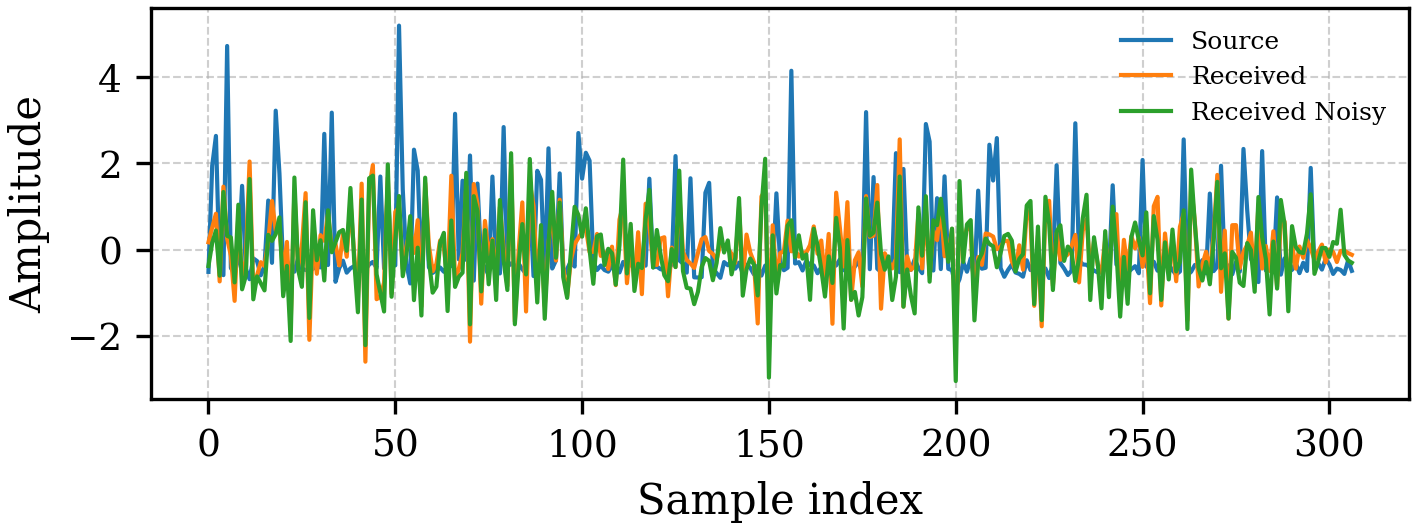
\includegraphics[width=\linewidth]{ltie_experiment1_all_signals_matplotlib.png}
\caption{The synthetic data used for experiment one- impulse response regression from a single observation.}
\label{fig:experiment1_a_all_data}
\end{figure}


\begin{figure}[!ht]
\centering
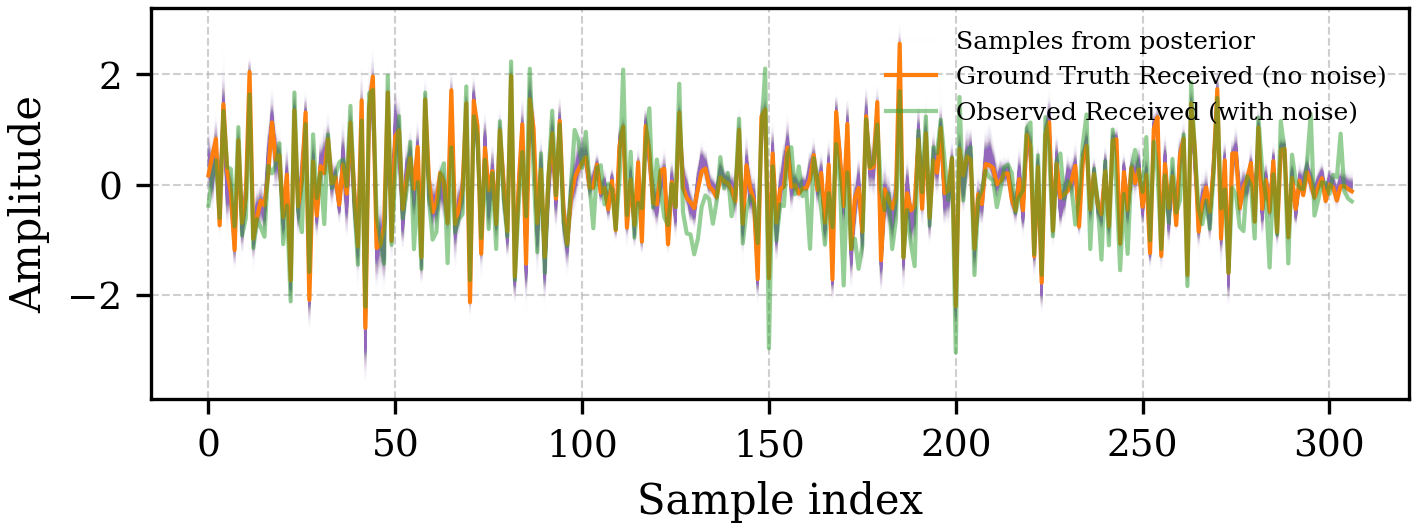
\includegraphics[width=\linewidth]{ltie_experiment1_samples_posterior_received_regression_vs_ground_truth_matplotlib.png}
\caption{Denoising performance of the Bayesian model in the single-observation experiment. The figure shows the posterior predictive distribution for the received signal, $\hat{g}[n]$ (a collection of green samples). By learning the impulse response, the model generates predictions that accurately reconstruct the clean signal while filtering the noise from the original observation.}
\label{fig:denoising_performance} 
\end{figure}


\begin{figure}[!ht]
    \centering
    \begin{subfigure}[b]{.47\linewidth}
        
\includegraphics[width=\linewidth]{ltie_experiment1_fir_estimate_matplotlib.png}
        \subcaption{The posterior mean (blue dashed line) of the estimated impulse response tracks the ground truth (orange). The shaded region indicates the epistemic uncertainty ($\pm 2$ standard deviations).}
        \label{fig:experiment1_a_samples_posterior_ir_estimate}
    \end{subfigure}
    \hfill
    \begin{subfigure}[b]{.47\linewidth}
        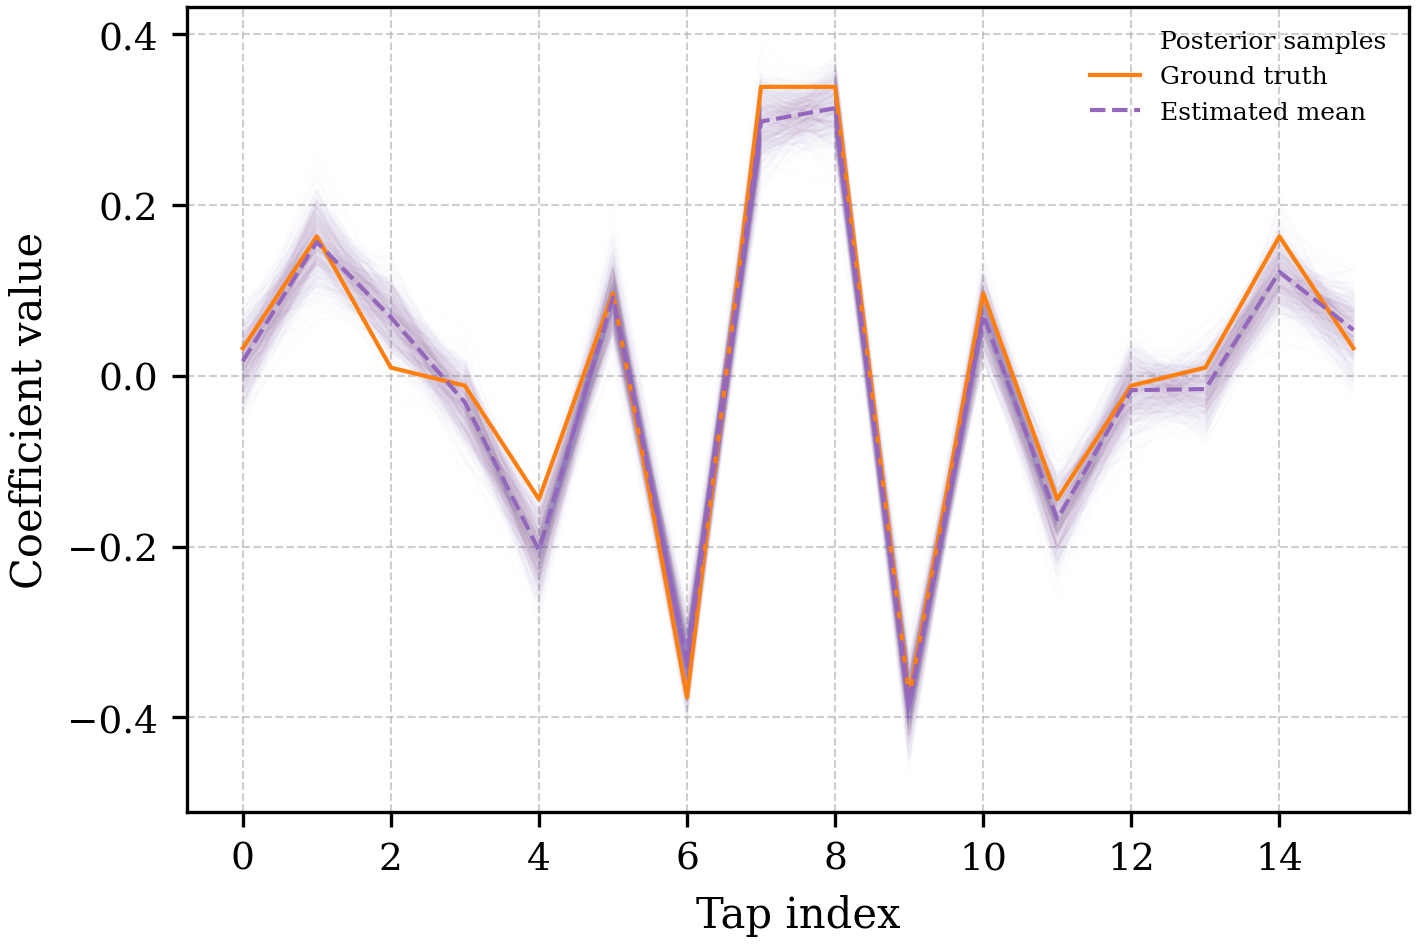
\includegraphics[width=\linewidth]{ltie_experiment1_samples_posterior_ir_matplotlib.png}
        \subcaption{Individual samples drawn from the posterior distribution (blue lines), illustrating the model's uncertainty around the ground truth impulse response (orange).}
        \label{fig:experiment1_a_samples_posterior_ir_samples}
    \end{subfigure}
    \caption{Bayesian estimation of the impulse response, $h[k]$, from a single noisy observation. The model learns a full posterior distribution that successfully recovers the ground truth filter and quantifies the associated estimation uncertainty.}
\end{figure}

\begin{figure}[!ht]
    \centering
        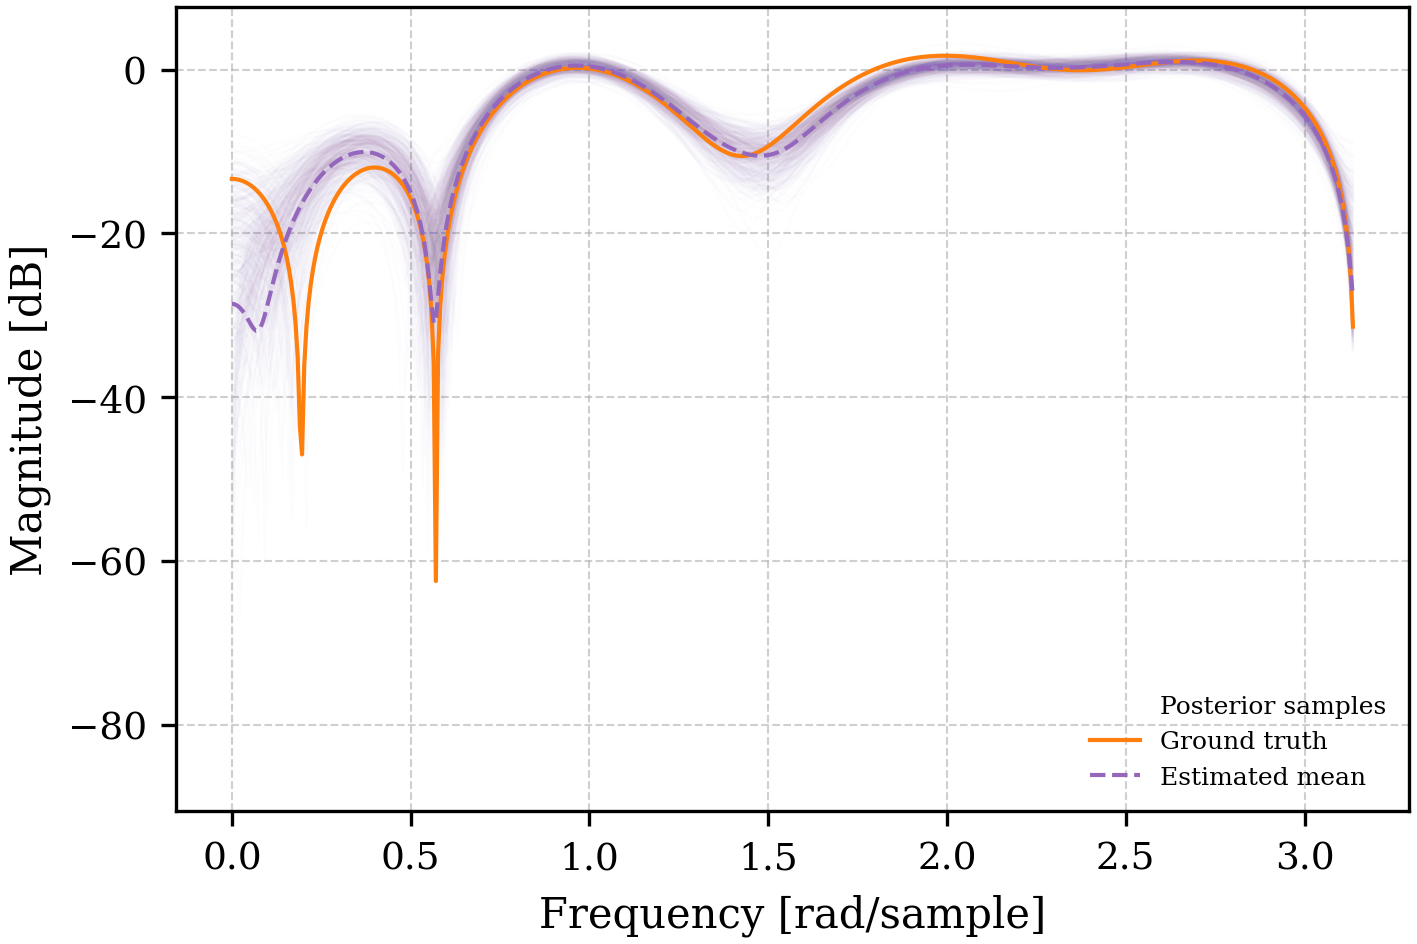
\includegraphics[width=\linewidth]{ltie_experiment1_samples_posterior_freq_matplotlib.png}
        
    \caption{Propagation of uncertainty into the frequency domain. The posterior distribution over the impulse response, $p(h \mid \mathcal{D})$, induces a full posterior over the system's frequency and phase response, allowing for comprehensive uncertainty analysis.}
    \label{fig:experiment1_a_samples_posterior_freq}
\end{figure}


\begin{figure}[!ht]
    \centering
    \begin{subfigure}[b]{0.48\textwidth}
        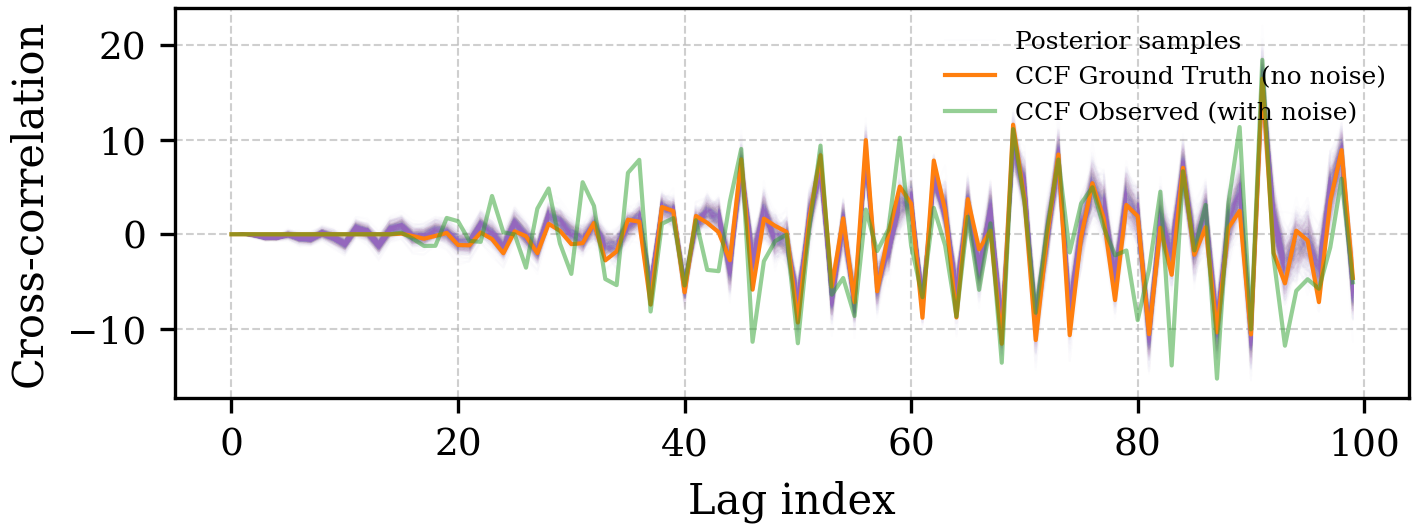
\includegraphics[width=\linewidth]{ltie_experiment1_samples_posterior_ccf_regression_vs_noisy_matplotlib_0.png}
        \subcaption{Zoom on lags near 0.}
        \label{fig:app:xcorr_zoom0}
    \end{subfigure}
    \hfill % Adds horizontal space
    \begin{subfigure}[b]{0.48\textwidth}
        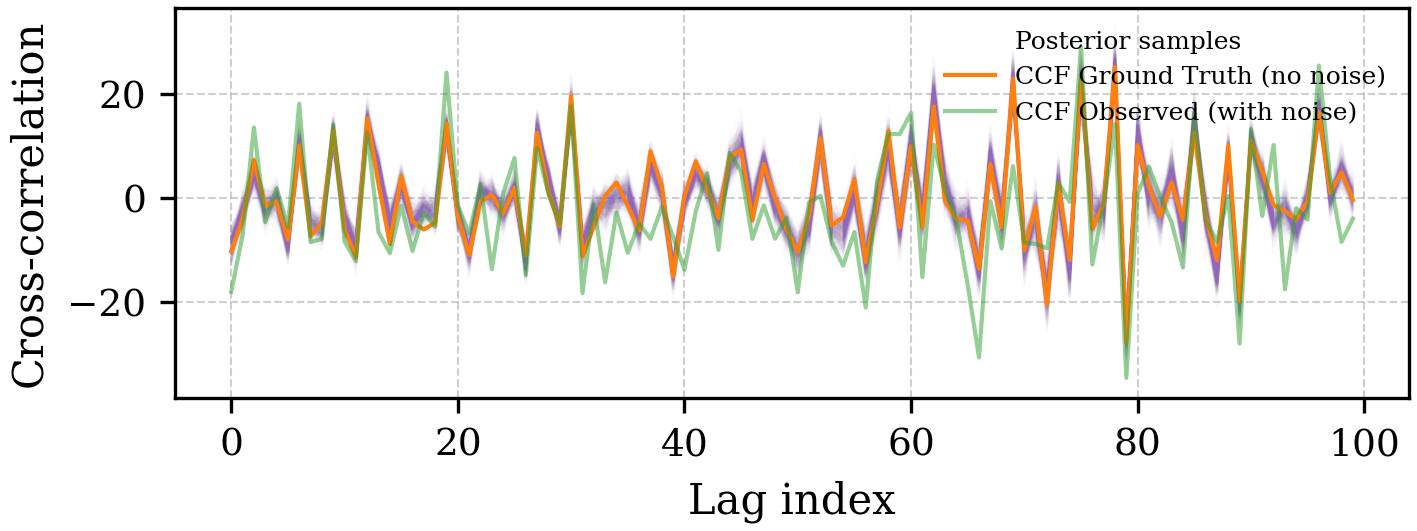
\includegraphics[width=\linewidth]{ltie_experiment1_samples_posterior_ccf_regression_vs_noisy_matplotlib_100.png}
        \subcaption{Zoom on lags near 100.}
        \label{fig:app:xcorr_zoom100}
    \end{subfigure}   
    
    \vspace{1em} % Adds some vertical space between rows

    \begin{subfigure}[b]{0.48\textwidth}
        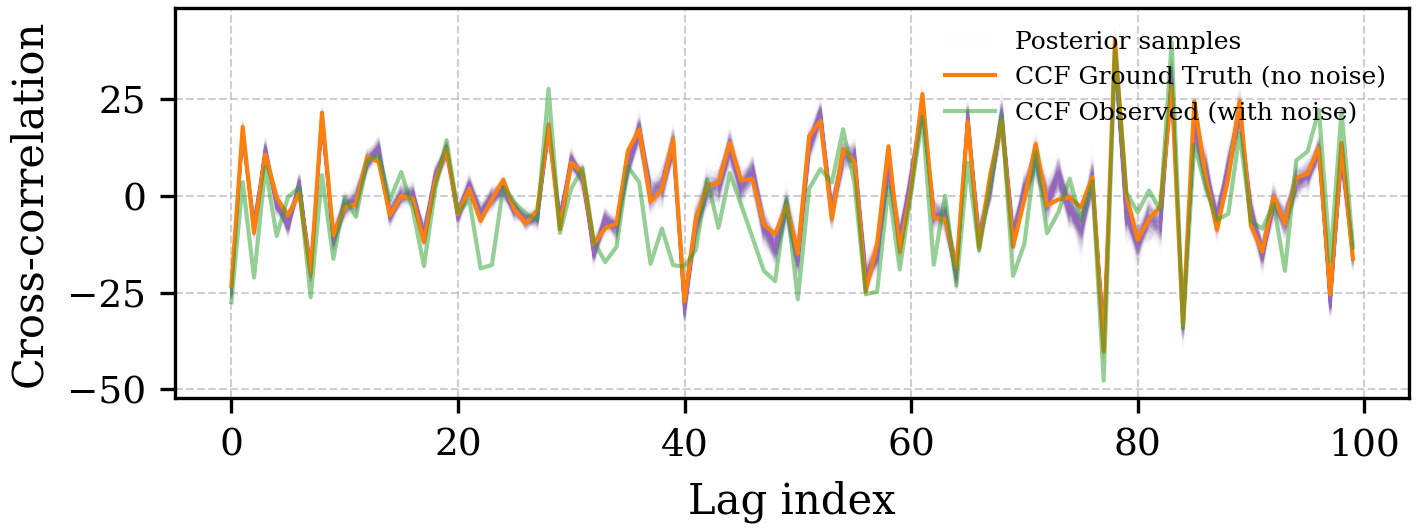
\includegraphics[width=\linewidth]{ltie_experiment1_samples_posterior_ccf_regression_vs_noisy_matplotlib_200.png}
        \subcaption{Zoom on lags near 200.}
        \label{fig:app:xcorr_zoom200}
    \end{subfigure}
    \hfill
    \begin{subfigure}[b]{0.48\textwidth}
        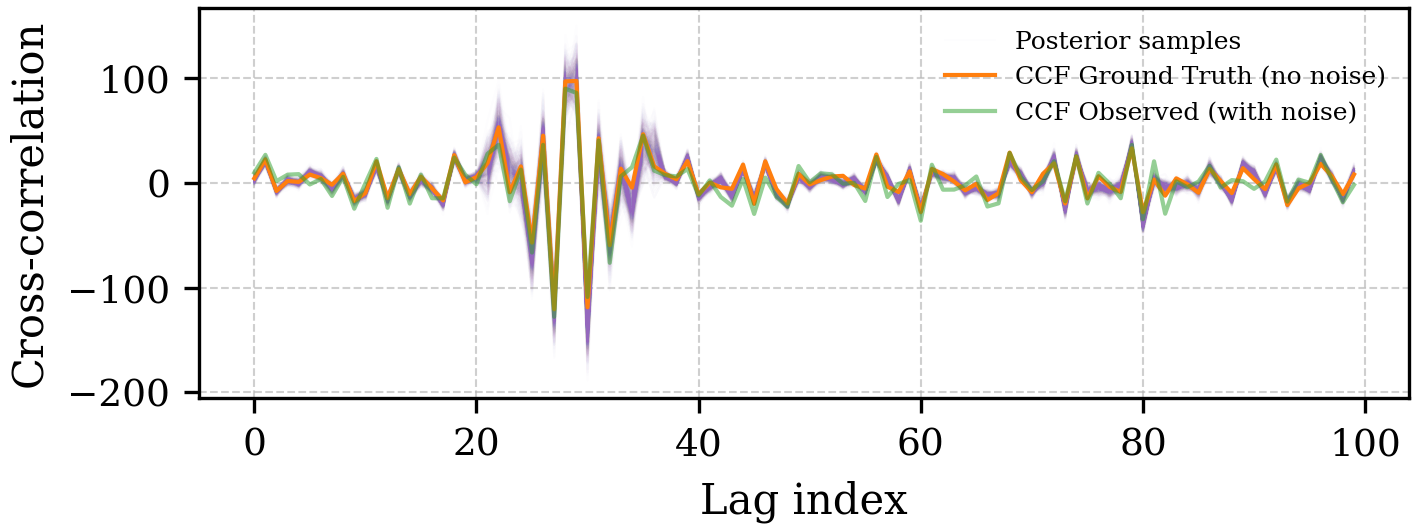
\includegraphics[width=\linewidth]{ltie_experiment1_samples_posterior_ccf_regression_vs_noisy_matplotlib_300.png}
        \subcaption{Zoom on lags near 300.}
        \label{fig:app:xcorr_zoom300}
    \end{subfigure} 
    
    \caption{Samples from the posterior distribution of the cross-correlation function (CCF) for the single-observation experiment. These plots show the estimated CCF distribution (green) robustly matching the ground truth (orange) while providing a credible interval, in contrast to the noisy observed CCF (red). Each panel shows a zoomed-in view of a different lag region.}
    \label{fig:app:xcorr_all} % A single label for the whole figure
\end{figure}

\clearpage

\section{Application to Simulated Ambient Noise Tomography}

\begin{figure}[!ht]
    \centering
    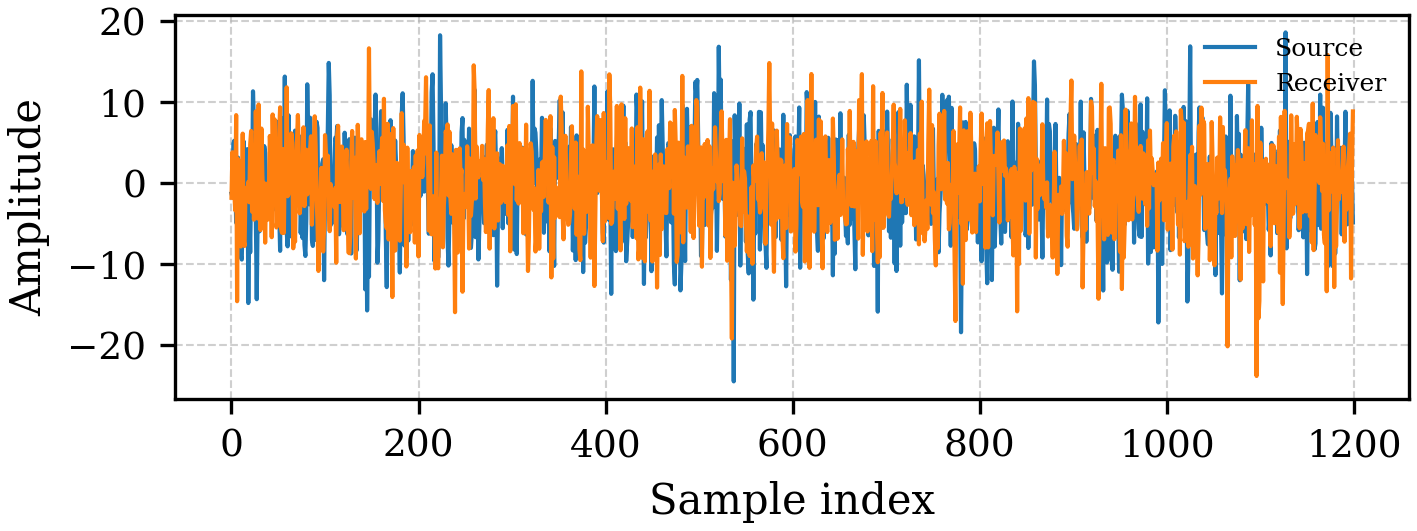
\includegraphics[width=\linewidth]{ant_pair_index_15_matplotlib.png}
    \caption{An example observation pair from the synthetic ANT simulation. Each signal represents the noisy superposition of waves from multiple sources, as recorded at two different receivers.}
    \label{fig:ant_example_pair}
\end{figure}

\begin{figure}[!h]
    \centering
    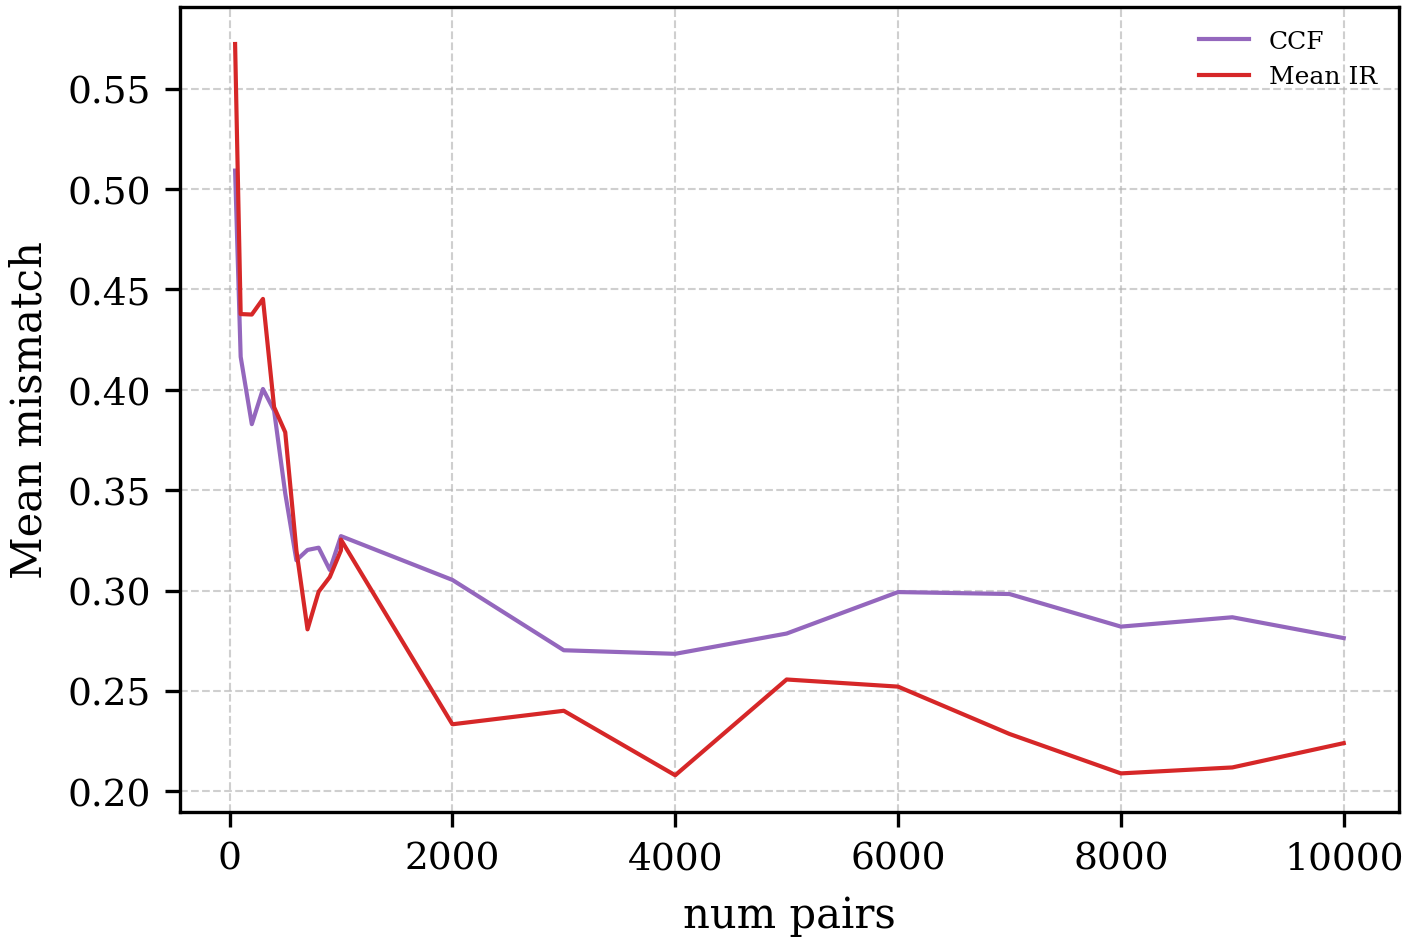
\includegraphics[width=0.8\textwidth]{ant_target_velocity_mean_mismatch_for_num_pairs_full_0.1_to-3.0_hz_matplotlib.png}
    \caption{Performance comparison showing target velocity mismatch error as a function of the number of signal pairs used. The Bayesian MIR method (red) demonstrates superior data efficiency, achieving a lower error with fewer observations and converging to a lower overall error floor compared to the classical CCF method (purple).}
    \label{fig:ant_error_vs_num_pairs}
\end{figure}

\begin{figure}[!h]
    \centering
    \begin{subfigure}[b]{.47\linewidth}
        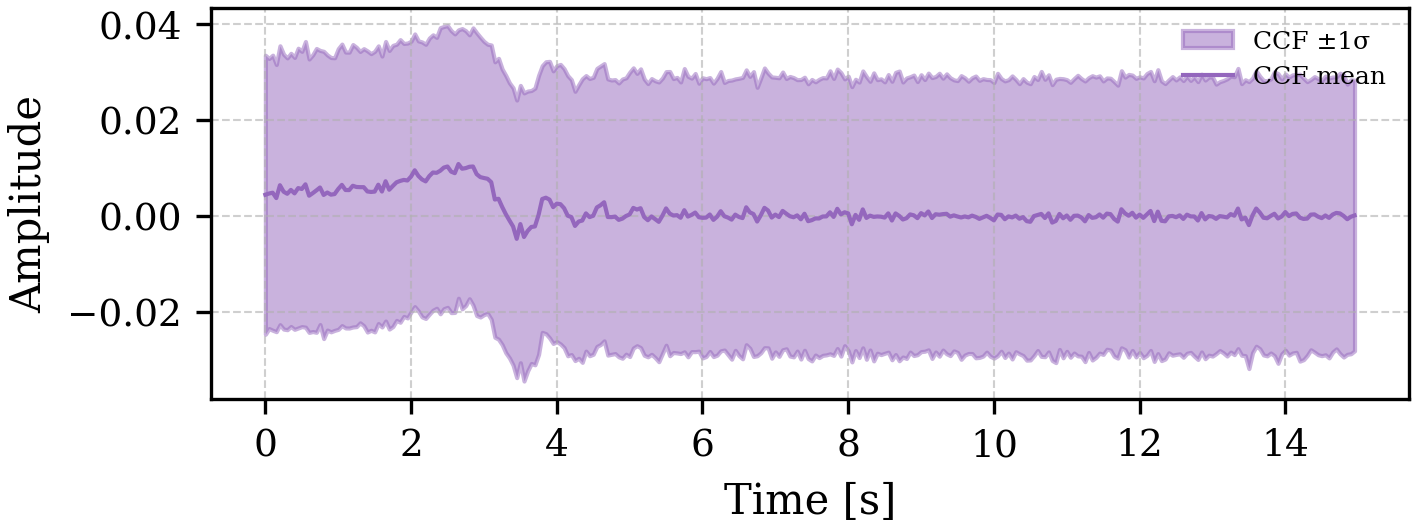
\includegraphics[width=\linewidth]{ant_estimated_ccf_full_right_half_matplotlib.png}
        \subcaption{The mean (purple) of the estimated Green's function computed by classical CCF stacking. The shaded region indicates the empirical standard deviation ($\pm 1 \sigma$).}
        \label{fig:ant_ccf_estimate}
    \end{subfigure}
    \hfill
    \begin{subfigure}[b]{.47\linewidth}
        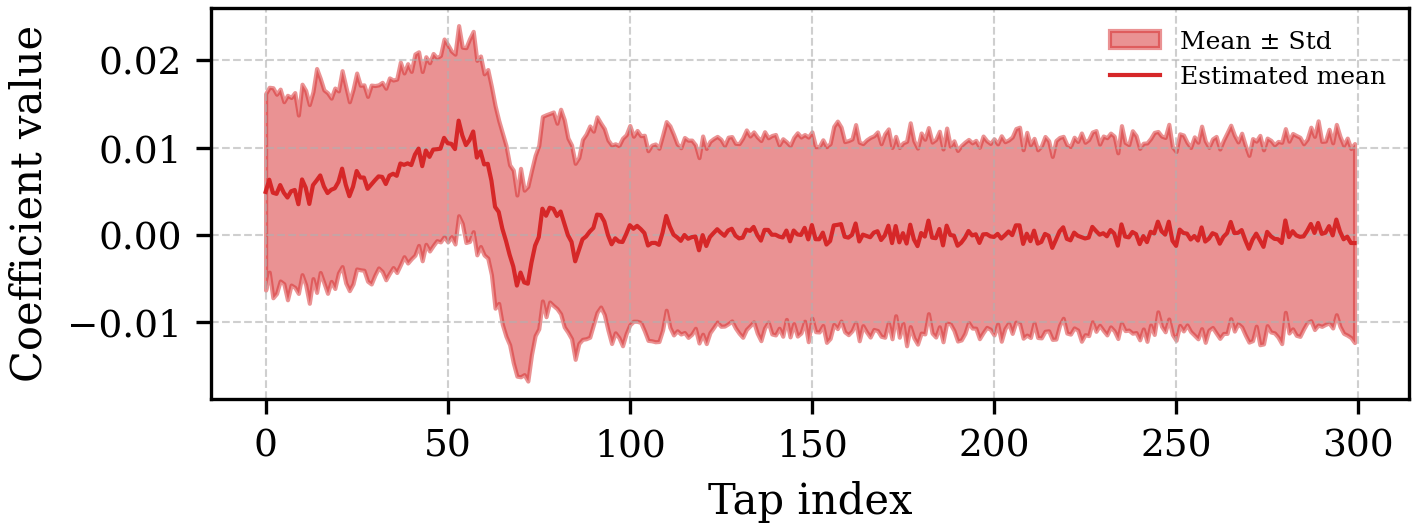
\includegraphics[width=\linewidth]{ant_estimated_ir_full_mean_right_half_matplotlib.png}
        \subcaption{The posterior mean (red) of the impulse response (Green's function) computed by our Bayesian model. The shaded region indicates the epistemic uncertainty ($\pm 1 \sigma$).}
        \label{fig:ant_mir_estimate}
    \end{subfigure}
    \caption{Comparison of the estimated Green's function from (a) classical CCF stacking and (b) our Bayesian model, using 2000 signal pairs. The Bayesian Mean Impulse Response (MIR) provides a smoother estimate of the arrivals and exhibits substantially lower uncertainty compared to the classical approach.}
\end{figure}

\begin{figure}[!h]
    \centering
    %--- Left Plot: Error vs. Frequency ---
    \begin{subfigure}[b]{0.48\textwidth}
        \centering
        
\includegraphics[width=\linewidth]{ant_cc_and_mir_full_error_by_freq_matplotlib.png}
        \caption{Velocity estimation error as a function of frequency for the classical CCF (purple) and Bayesian MIR (red) methods. The MIR method shows lower error across most frequency bands.}
        \label{fig:ant_error_vs_freq}
    \end{subfigure}
    \hfill % Adds horizontal space between figures
    %--- Right Plot: Relative Uncertainty ---
    \begin{subfigure}[b]{0.48\textwidth}
        \centering
        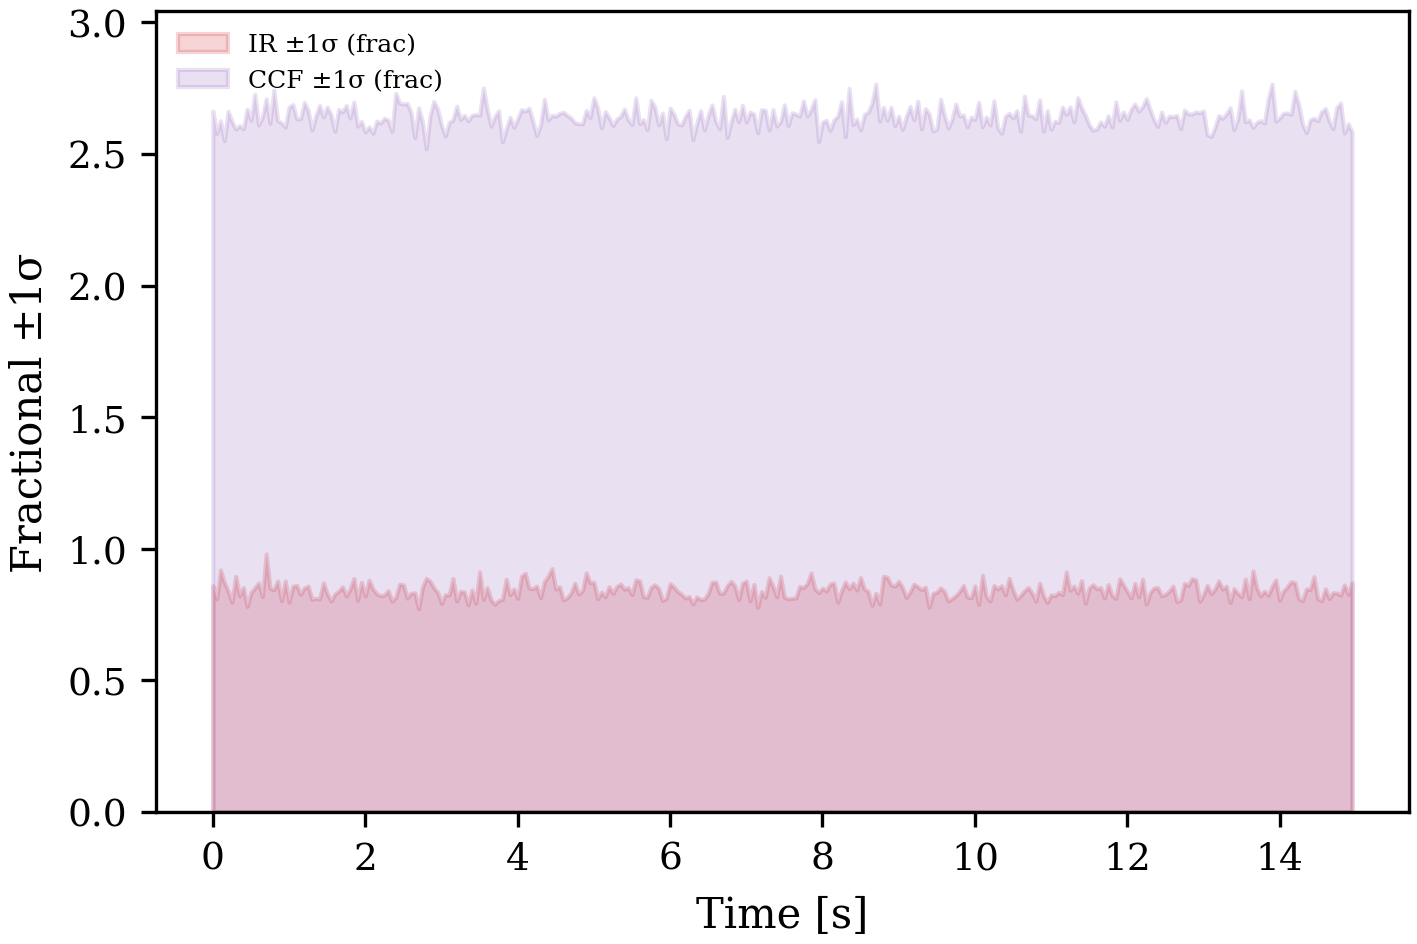
\includegraphics[width=\linewidth]{ant_estimated_ir_and_ccf_full_relative_uncertainty_matplotlib.png}
        \caption{Relative uncertainty (standard deviation divided by magnitude) for both impulse response estimates. The Bayesian MIR (red) exhibits significantly lower uncertainty.}
        \label{fig:ant_relative_uncertainty}
    \end{subfigure}
    \caption{Quantitative performance comparison of the classical CCF and Bayesian MIR methods using 2000 signal pairs. The Bayesian approach achieves (a) lower velocity estimation error across the spectrum and (b) is characterized by substantially lower relative uncertainty.}
    \label{fig:ant_quantitative_comparison}
\end{figure}

\begin{figure}[!htp]
    \centering
    %--- Top Plot: CCF Misfit Map ---
    \begin{subfigure}{0.75\textwidth}
        \centering
        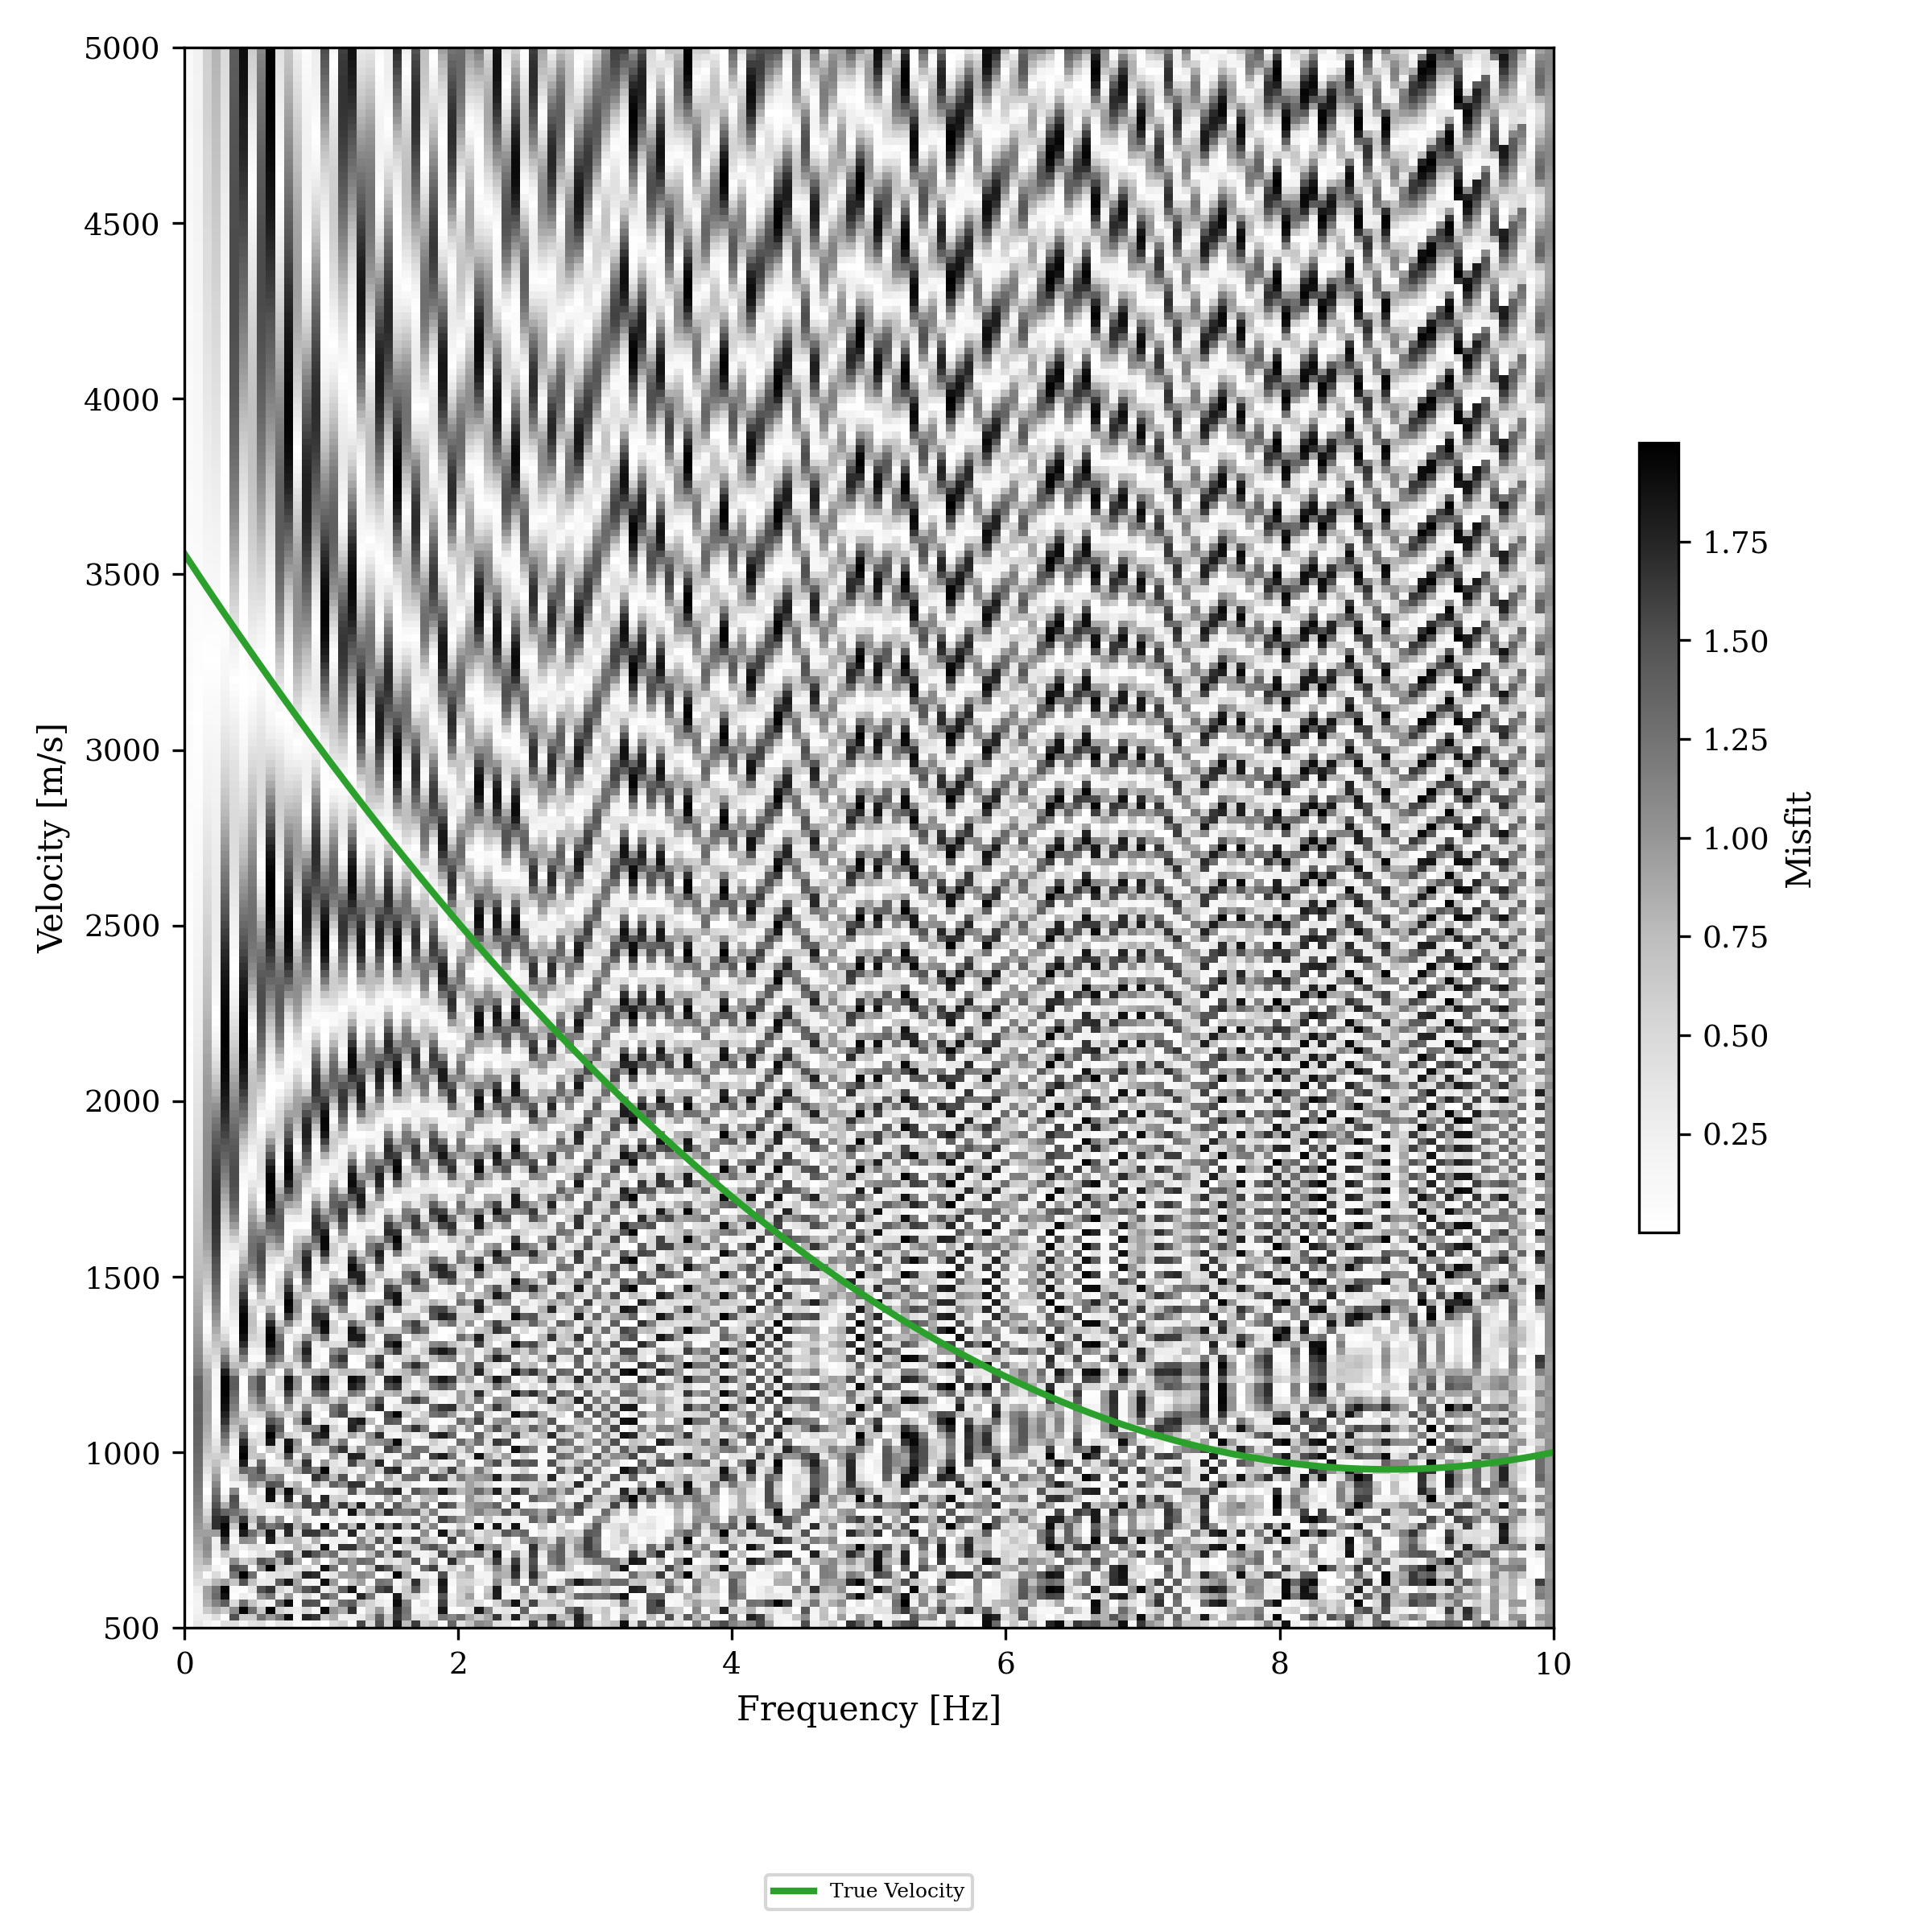
\includegraphics[width=\linewidth]{ant_estimated_cc_full_velocity_misfit_matplotlib.png}
        \caption{Velocity misfit map for the classical CCF estimate. The green line is the ground-truth velocity.}
        \label{fig:ant_misfit_map_ccf}
    \end{subfigure}
    
    \medskip % Adds some vertical space between the plots

    %--- Bottom Plot: MIR Misfit Map ---
    \begin{subfigure}{0.75\textwidth}
        \centering
        
\includegraphics[width=\linewidth]{ant_estimated_mir_full_velocity_misfit_matplotlib.png}
        \caption{Velocity misfit map for the Bayesian MIR estimate. The green line is the ground-truth velocity.}
        \label{fig:ant_misfit_map_mir}
    \end{subfigure}
    
    \caption{Comparison of velocity misfit maps for (a) the classical CCF and (b) the Bayesian MIR methods. The misfit (error) is shown in greyscale, where darker shades indicate higher error. The Bayesian MIR shows a lower error margin around the ground-truth velocity curve (green), particularly at lower frequencies, and its low-misfit valley extends more smoothly into the higher frequency range (up to 3Hz). This leads to a more accurate and robust final velocity estimation.}
    \label{fig:ant_misfit_maps_comparison}
\end{figure}

\clearpage

\section{Regression of a Non-Stationary Impulse Response}

\begin{figure}[!ht]
    \centering
    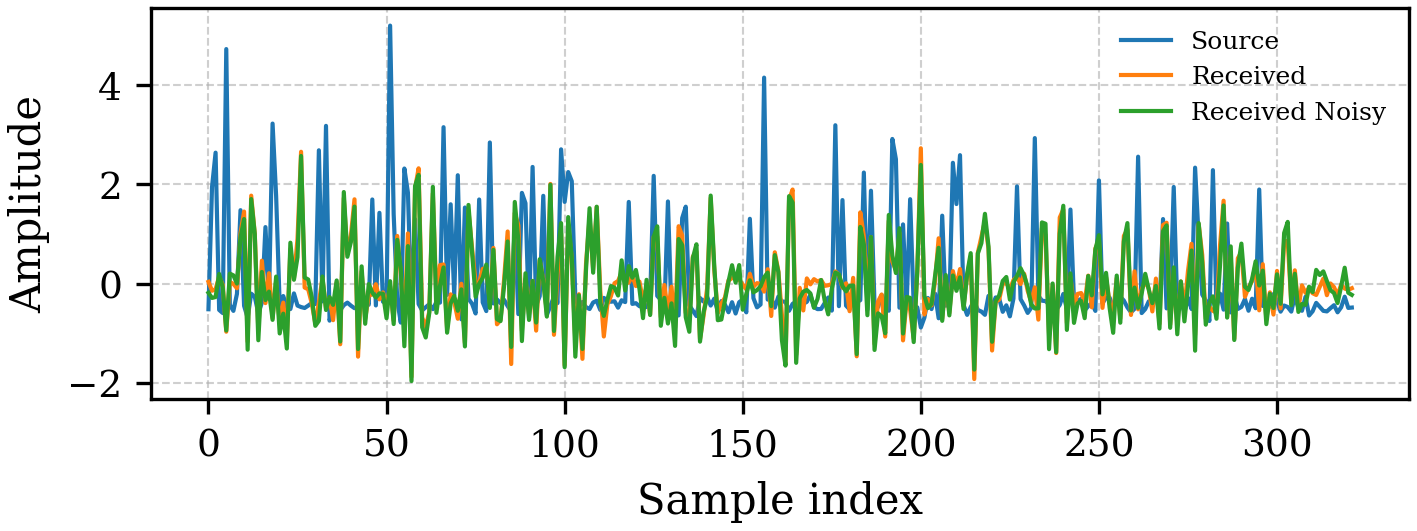
\includegraphics[width=\linewidth]{ltv_experiment1_all_signals_matplotlib.png}
    \caption{Synthetic data for the LTV system identification experiment. The figure shows: the input signal $s[n]$, the ground-truth time-varying impulse response $h[n, k]$, and the resulting noisy output signal $r[n]$.}
    \label{fig:ltv_experiment1_example_pair}
\end{figure}

\begin{figure}[!ht]
    \centering
    \begin{subfigure}[b]{.47\linewidth}
        \centering
        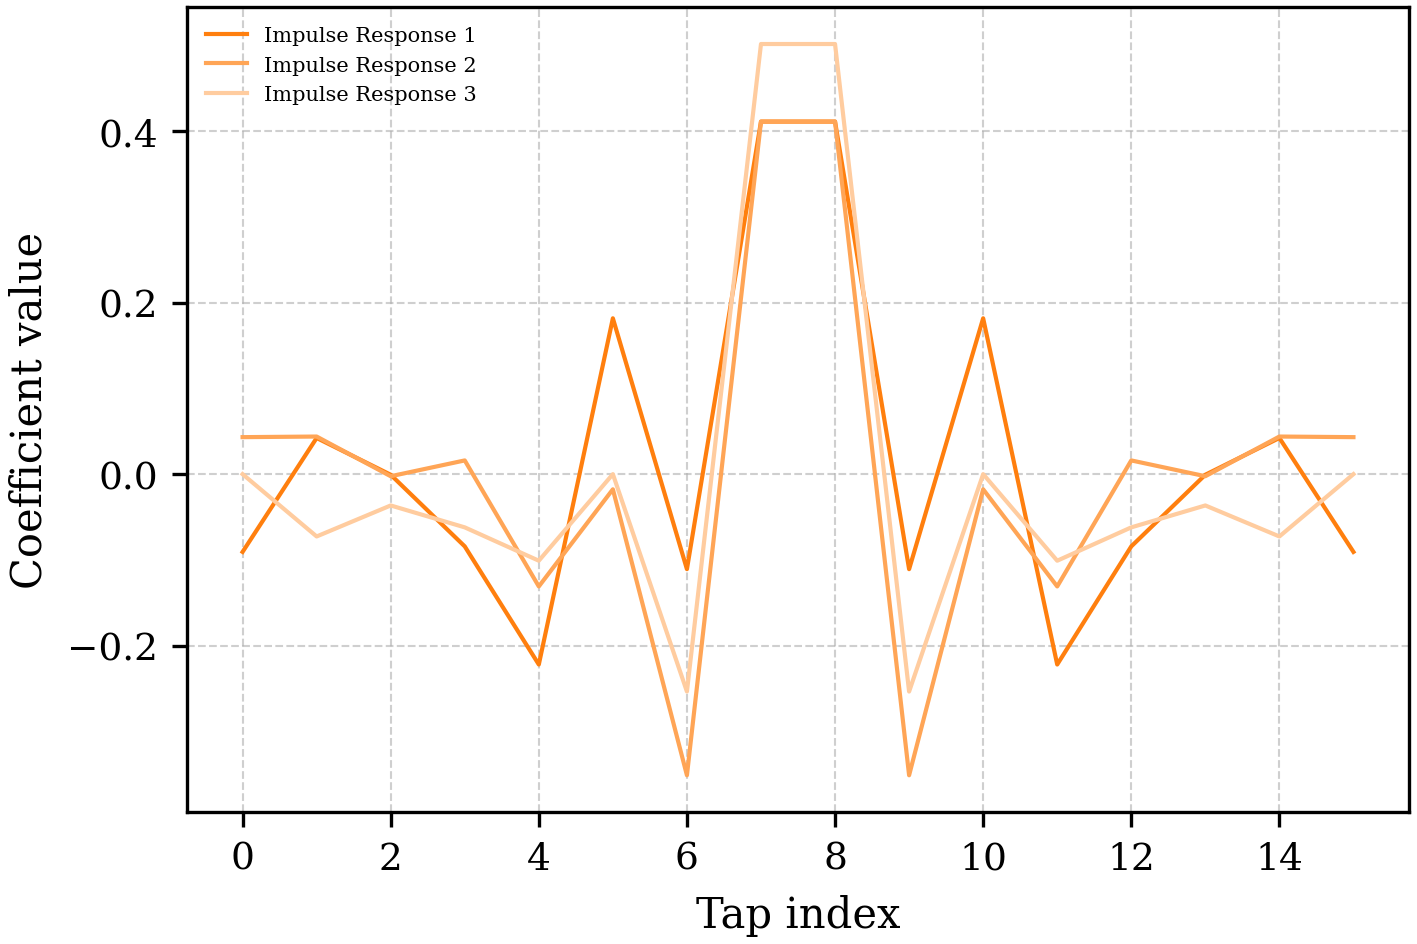
\includegraphics[height=3.8cm, keepaspectratio]{ltv_experiment1_fir_ground_truth_components_matplotlib.png}
        \subcaption{The three distinct time-invariant FIR filters that serve as the basis for the LTV system.}
        \label{fig:ltv_experiment1_three_fir_components}
    \end{subfigure}
    \hfill
    \begin{subfigure}[b]{.47\linewidth}
        \centering
        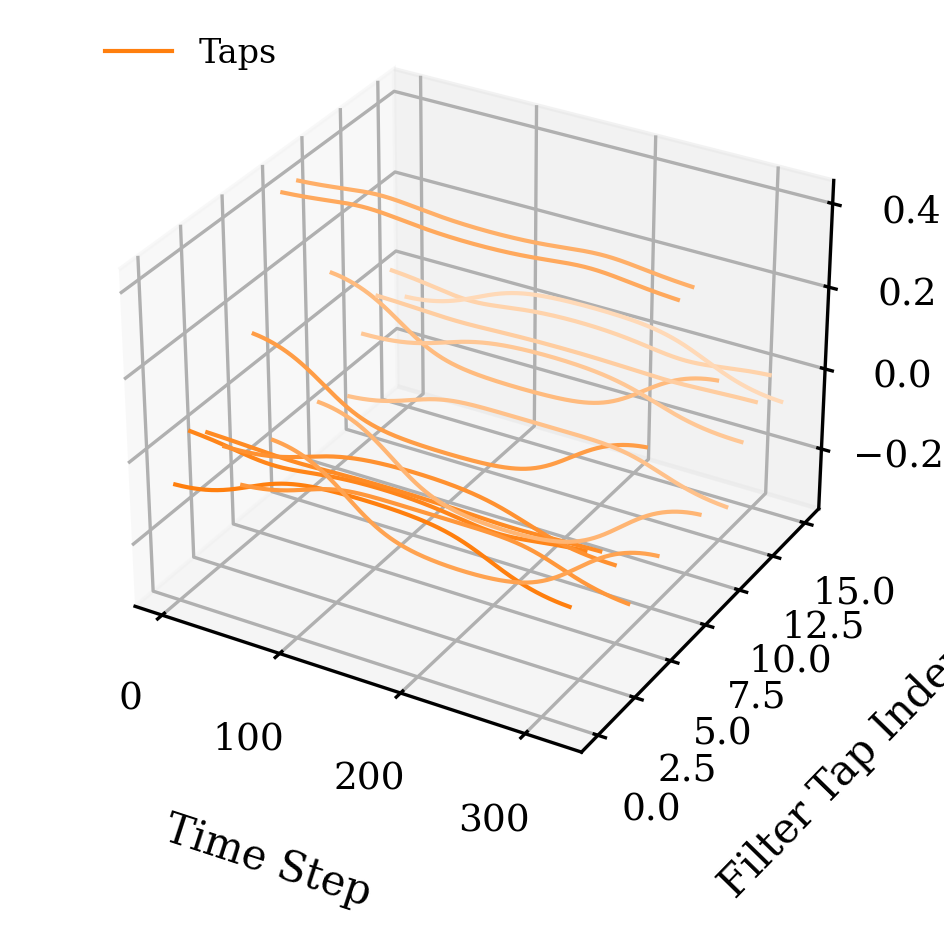
\includegraphics[height=4cm, keepaspectratio]{ltv_experiment1_ltv_fir_ground_truth_3d_matplotlib.png}
        \subcaption{The final time-varying impulse response created by smoothly interpolating between the three base filters over time.}
        \label{fig:ltv_experiment1_a_samples_posterior_ir_samples}
    \end{subfigure}
    \caption{Generation of the ground-truth time-varying impulse response, $h[n, k]$. The LTV system is synthesized by smoothly interpolating between the three distinct FIR components shown in (a) to produce the final time-varying response shown in (b).}
    \label{fig:ltv_ground_truth_generation}
\end{figure}

\begin{figure}[!ht]
    \centering
    \begin{subfigure}[b]{.47\linewidth}
        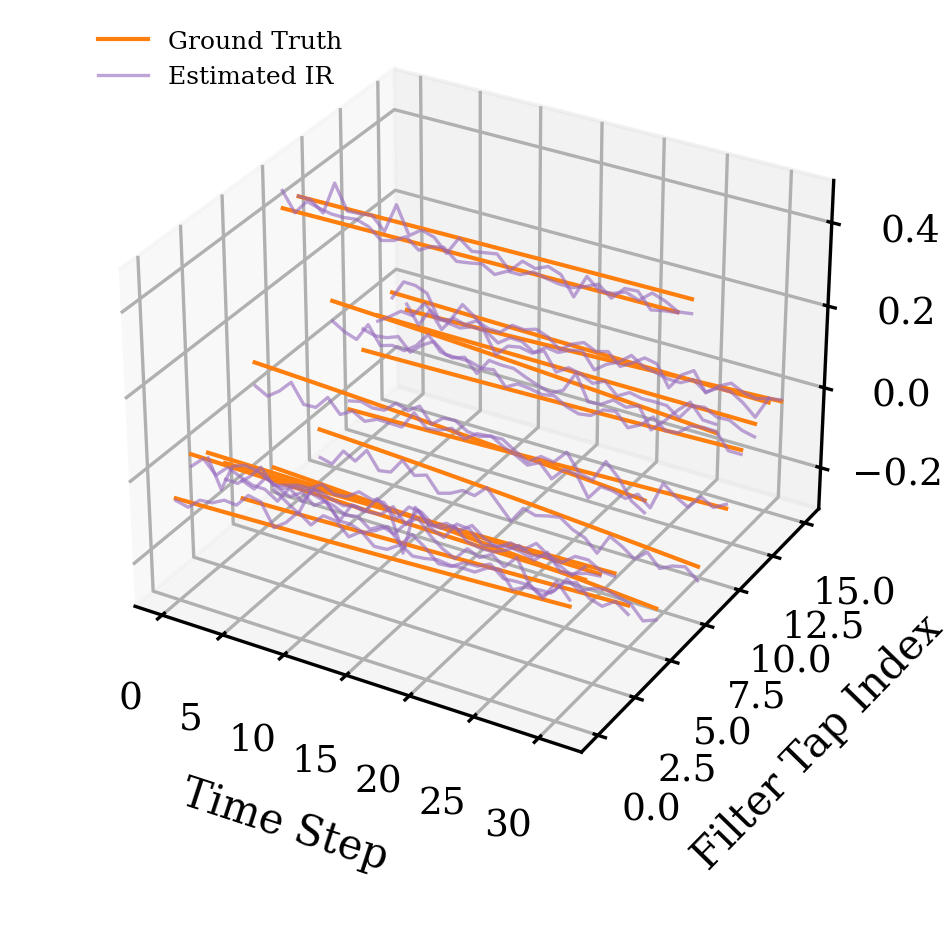
\includegraphics[width=\linewidth]{ltv_single_plot_fir_fit_and_ground_truth_matplotlib.png}
        \subcaption{The estimated FIR (purple) and ground truth (orange) for a single time window. The smoothness of the estimate within this window is regularized by the Gaussian Process prior.}
        \label{fig:ltv_experiment1_single_window_fit}
    \end{subfigure}
    \hfill
    \begin{subfigure}[b]{.47\linewidth}
        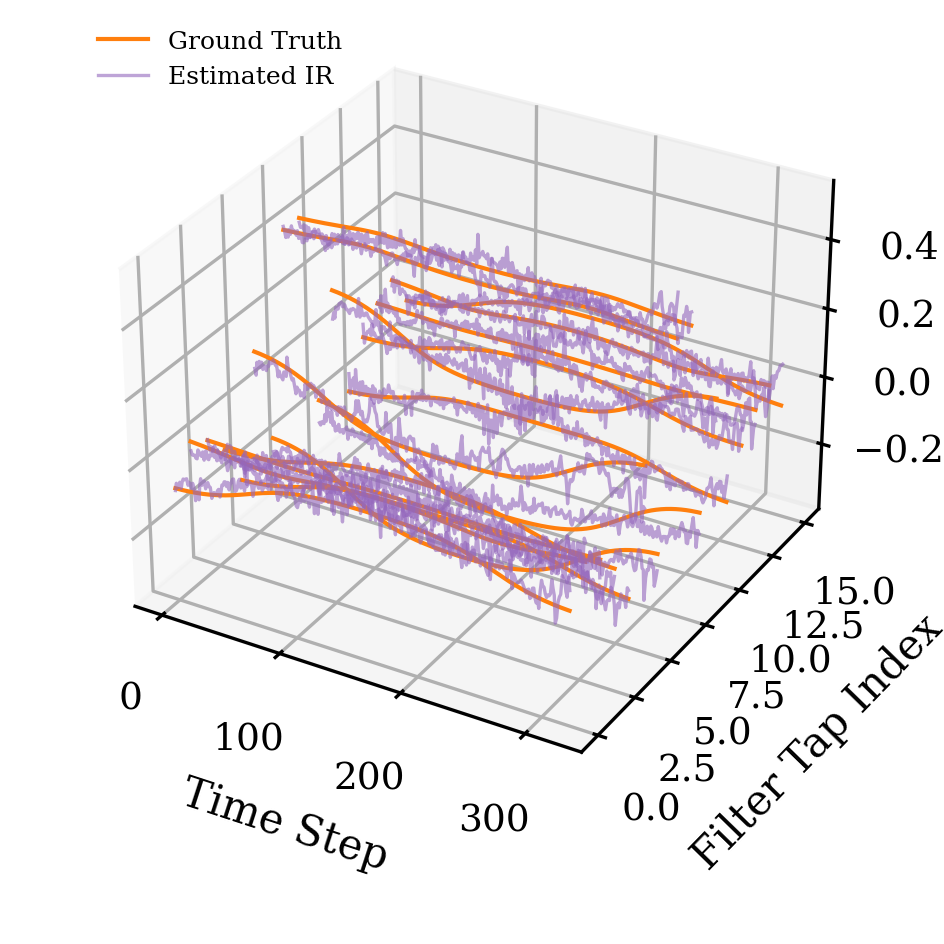
\includegraphics[width=\linewidth]{ltv_stitched_plot_fir_fit_and_ground_truth_matplotlib.png}
        \subcaption{The complete LTV impulse response estimate (purple), created by averaging the predictions from all overlapping windows, shown against the ground truth (orange).}
        \label{fig:ltv_experiment1_stitched_fit}
    \end{subfigure}
    \caption{Estimation of the time-varying impulse response, $h[n, k]$. (a) The model's estimate for a single time window. (b) The complete LTV response, reconstructed by stitching together the estimates from all overlapping windows. The final result successfully tracks the ground-truth system dynamics.}
\end{figure}

\end{document}